\documentclass{pclass}
\usepackage [spanish] {babel} 
\usepackage[utf8]{inputenc}
\usepackage{eurosym}
\usepackage{graphicx}
\usepackage{float}
\usepackage{url}
\begin{document}
\pagenumbering{arabic}
\tipo{Grado}   % Grado o M\'aster
\titulopro{Control de un coche mediante Raspberry Pi}
\tutor{Manuel Jesús Domínguez Morales}
\departamento{Arquitectura y Tecnología de Computadores}
%\autores{Nombre 1}{Nombre 2}  % Dos autores
\autores{Gonzalo Romero Castillo}{{\ }}   % Un autor
\dia{26 de Junio de 2017 (v.1.0)}
\titulacion{GITI}

\hacerportada

	\makeatletter
\renewcommand*\l@section{\@dottedtocline{1}{0em}{2.5em}}
\renewcommand*\l@subsection{\@dottedtocline{2}{1.5em}{3.2em}}
\renewcommand*\l@subsubsection{\@dottedtocline{3}{4.3em}{3.2em}}
\makeatother

\renewcommand{\frontmatter}{\pagenumbering{Roman}}
\frontmatter

\cdpchapter{Agradecimientos}

Mis más sinceros agradecimientos a:

\begin{itemize}
	\item Ángel Suárez Mora
	\item Francisco Javier Fernández Rodríguez
	\item Manuel Jesús Domínguez Morales
	\item Felix Romero Romero
	\item Petra Castillo Herrera
	\item Ángela Romero Castillo
	\item Juan Manuel Gutierrez Romero
	\item Jose Antonio (Villa)
	\item Antonio Cordero Sánchez
	
\end{itemize}
 
\cdpchapter{Resumen}

\cdpchapter{Resumen en inglés}
        
	\tableofcontents


	\listoffigures
\mainmatter  


\chapter{BLOQUE 1: DESCRIPCI\'ON DEL PROYECTO}
\section{Introducci\'on y motivaci\'on}
\section{Objetivos del proyecto}
\section{Estado del arte}
El radio control nace en 1894 de la mano de Guillermo Marconi, el cual, realizó un experimento en el cual se accionaba una campanilla sin necesidad de hacer uso de un cable de cobre como en el telégrafo, muy usado en esa época. Este experimento no hubiese sido posible sin que antes otros cientificos como Maxwell, teoría de la existencia de las ondas electromagnéticas, Hertz, experimentos centrados en la emisión de descargas, y Rumkorff no hubiesen descubierto los fenómenos de radiación e inducción.

En 1940, en plena II Guerra Mundial, surge un primer proyecto en el cual se dotaba a un avión de un sistema de radiocontrol. La idea de aviones radiodirigidos surge para intentar ahorrar vidas, ya que el avion, una vez puesto en el aire, era controlado desde tierra. Con el paso de los años, la mejora en los circuitos integrados y la miniaturización de estos, se incluye el radiocontrol en el modelismo. Aquí es donde este trabajo puede ser clasificado, en el modelismo de radiocontrol, aunque con algunos matices.

En el mercado existen infinidad de coches de modelismo radiocontrol controlados por una emisora y un receptor de ondas de radio. En este caso, se trata de un sistema en el que se utiliza la conectividad wifi para controlar el modelo, lo cual nos hace que el control pueda ser un dispositivo variable. Existen en el mercado algunos productos similares a este, como son modelos controlados desde un móvil a través de la conección Bluetooth. La idea de este sistema es dotar al sistema de un sistema no tan rígido como un sistema de tiempo real, si no de un computador capaz de ser programado incluso para automatizar el control del modelo. A continuación mostramos varios productos ya existentes:



\begin{itemize}
    \item Spy Tank


\begin{figure}[H]
  \centering
    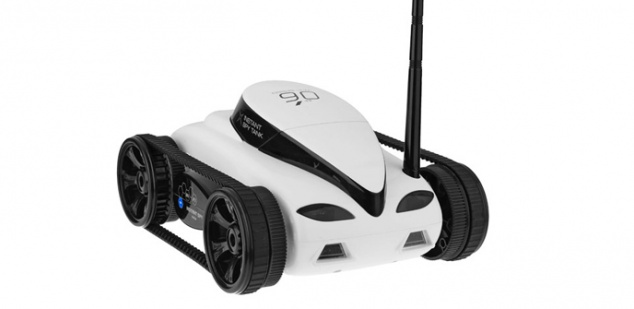
\includegraphics[width=1.1\textwidth]{img/producto1}
  \caption{Spy Tank}
  \label{fig:SpyTank}
\end{figure}



Este producto, el cual está diseñado para espiar, no para el disfrute del modelismo, tiene como puntos a favor que añade visión nocturna, camara de visión con 360º, micrófono y altavoz. Tienen a su disposición sendas aplicaciones para Android e iOS, en las que con un uso sencillo de la interacción con la app es fácil controlar el coche, como por ejemplo con los acelerometros. Por contra, para el uso de este dispositivo necesitamos de una red wifi existente, ademas de su precio, unos 150 \euro más gastos de envío.



    \item BMW X6 Bluetooth
\end{itemize}

\begin{figure}[H]
  \centering
    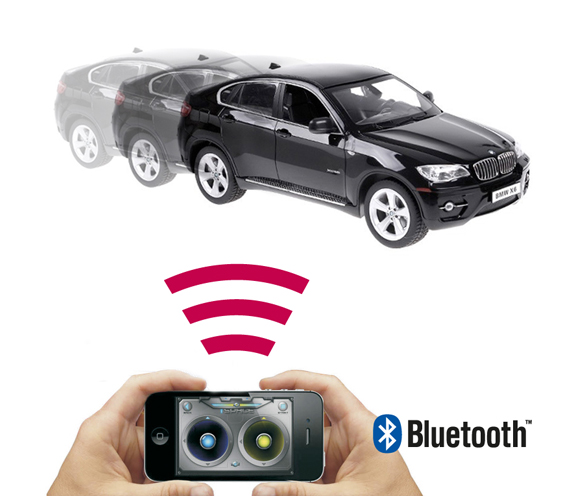
\includegraphics[width=1.1\textwidth]{img/producto2}
  \caption{BMW X6}
  \label{fig:BMWX6}
\end{figure}


Este producto se parece más a nuestro proyecto, podemos disfrutar del modelismo a un muy buen precio que ronda los 50 \euro. Simplemente nos encontramos con un coche que podemos controlar con sendas aplicaciones Android e iOS con la conexión Bluetooth. Por contra, no usa la red wifi, no tiene camara de visión y además es tan simple que no podríamos implementar nada ya que no contiene ningún sistema programable con el que poder eliminar esa rigidez.



\section{Elicitaci\'on de requisitos y an\'alisis de riesgos}
\chapter{BLOQUE 2: EJECUCI\'ON DEL PROYECTO}
\section{Diseño del sistema} 
\section{Implementación} 
\subsection{Tecnologías empleadas}

\begin{itemize}
	\item Hardware
		\begin{itemize}
			\item Raspberry Pi 3
			\item Arduino Nano
			\item Webcam
			\item Variador
			\item Servo
		\end{itemize}
	\item Software
	\begin{itemize}
		\item Mjpg Streamer
		
		MJPG-Streamer es un aplicación que se ejecuta por línea de comandos. A grandes rasgos, se encarga de obtener frames JPG (imágenes) capturadas desde una cámara compatible y transmitirlas como M-JPEG (secuencia de vídeo) mediante el protocolo HTTP para poder visualizarlo en navegadores, VLC y otras herramientas.
			\cite{mjpg}
		
		\item Hostapd y udhcpd
		
		Hostapd es un daemon para crear puntos de acceso y servidores de autentificación. Puede ser utilizado para crear puntos de acceso usando un ordenador con Linux. 
		
		Udhcpd es un pequeño servidor DHCP orientado a los sistemas embebidos.
		
			\cite{wireless}
		
		\item Raspbian	
		
		Raspbian es el sistema operativo oficial de la fundación Raspberry. Raspbian viene preinstalado con un montón de software para la educación, programación y uso general. Tiene Python, Scratch, Sonic Pi, Java, Mathematica y mucho más. En la versión lite no se usa interfaz gráfica.
		
			\cite{raspbian}
				
	\end{itemize}
	\item Lenguajes
		\begin{itemize}
			\item Python
			\item Arduino
			\item Java
		\end{itemize}
	\item Software de desarrollo
	\begin{itemize}
		\item Spyder
		\item Android Studio
		\item Arduino IDE
		\item Fritzing
		
		Fritzing es una iniciativa de hardware de código abierto que hace que la electrónica sea accesible como un material creativo para cualquiera. Ofrecemos una herramienta de software, un sitio web comunitario y servicios en el espíritu de Processing y Arduino, fomentando un ecosistema creativo que permite a los usuarios documentar sus prototipos, compartirlos con otros, enseñar electrónica en un aula y diseñar y fabricar PCB profesionales.
			\cite{fritzing}
		
		\item Tinkercad
		
		Tinkercad es una sencilla herramienta de diseño y modelado 3D basada en navegador que todos pueden usar. Tinkercad permite a los usuarios diseñar en cuestión de minutos todo lo que puedan imaginar.
			\cite{tinkercad}
			
		\item TeXstudio
		
		Texstudio es un entorno de escritura integrado para la creación de documentos LaTeX. Nuestro objetivo es hacer que la escritura del látex lo más fácil y cómoda posible. Por lo tanto texstudio tiene numerosas características como resaltado de sintaxis, visor integrado, verificación de referencias y varios asistentes.
			\cite{texstudio}
		\item Photoshop
		\item Gliffy
		
		Gliffy es una herramienta online que permite la creación de diferentes tipos de diagramas profesionales de forma sencilla.
			\cite{gliffy}
		
	\end{itemize}
\end{itemize}

 
\subsection{Desarrollo}

\begin{itemize}

\item Hardware y prototipo

En primer lugar, se llevó a cabo el desmontaje de las piezas innecesarias del prototipo, para sustituir las adecuadas para este sistema. En primer lugar se eliminó el antiguo receptor/variador para ser remplazado por un variador que controlase el motor sin ningún tipo de problemas. A esto se le sumó un problema, el servomotor que el prototipo traía era un motor eléctrico continuo, con lecturas de un potenciómetro, lo que después de muchas pruebas, tuvo que ser descartado dado que las lecturas del potenciómetro eran muy oscilantes e imposibilitaban el manejo correcto de la dirección. Siendo así, se sustituyo este servomotor, por un micro-servomotor normal, con el cual es mucho más fácil de trabajar.
A continuación se mostrará el coche sin ningún tipo de modificación:

\begin{figure}[H]
  \centering
    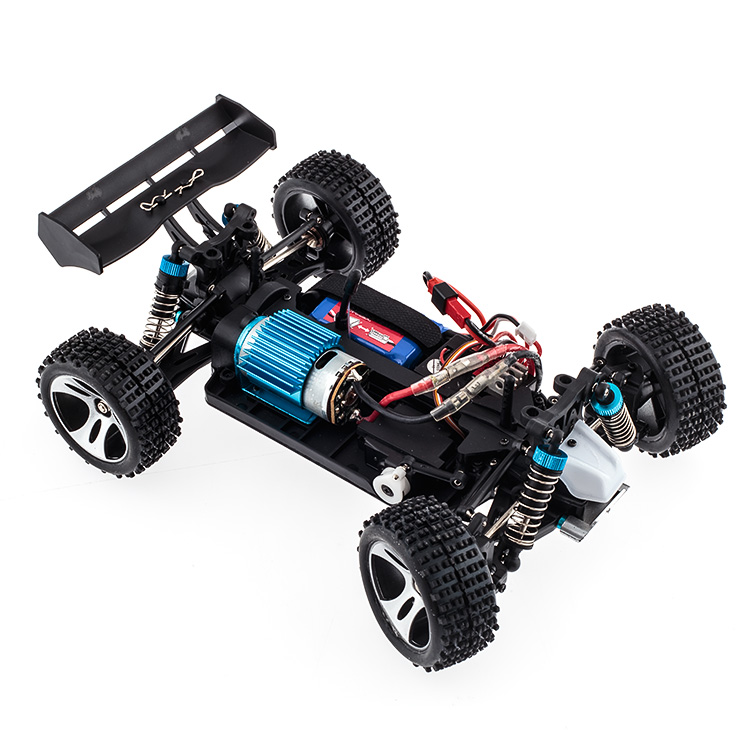
\includegraphics[width=0.7\textwidth]{img/A959}
  \caption{Coche sin desmontar}
  \label{fig:CocheSin}
\end{figure}

En la siguiente figura, se muestran las piezas elminadas del prototipo:

\begin{figure}[H]
  \centering
    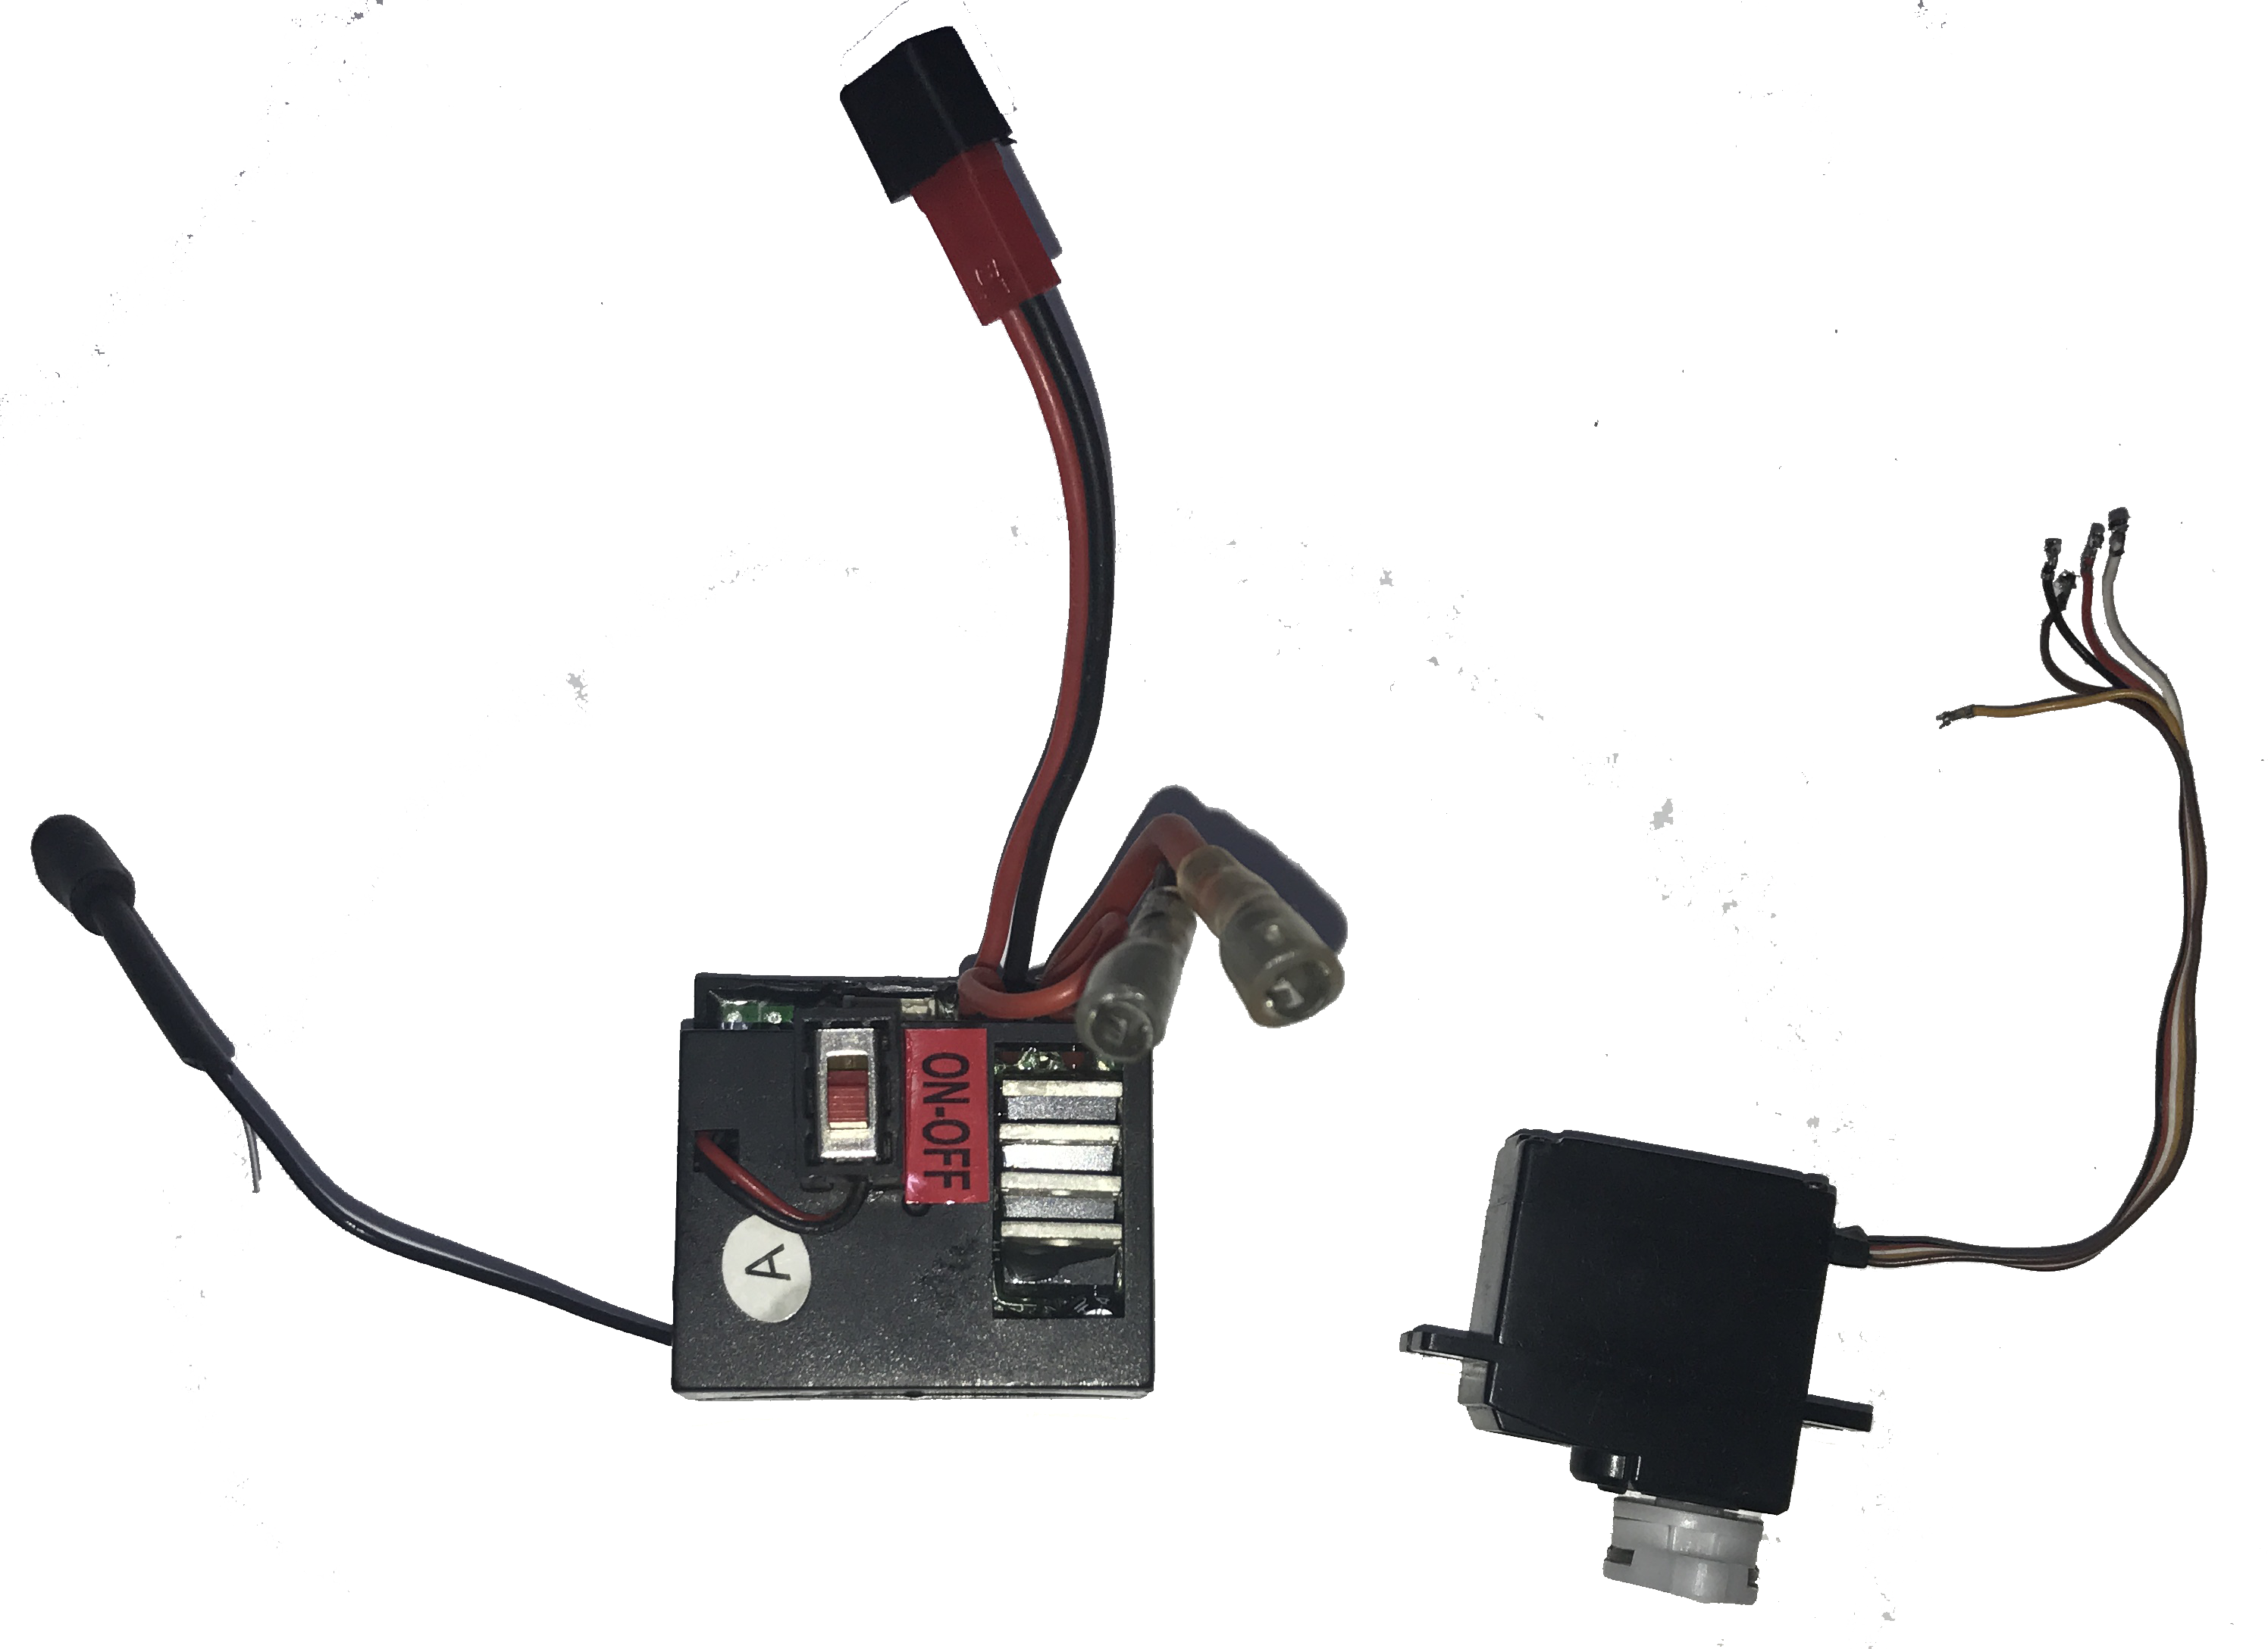
\includegraphics[width=0.7\textwidth]{img/piezasSustituidas}
  \caption{Piezas sustituidas}
  \label{fig:PiezasSusti}
\end{figure}

En la imagen que sigue, se muestra el prototipo con las nuevas piezas instaladas en su ubicación final. El variador lo encontramos en la parte frontal izquierda y el servomotor de la dirección en la parte frontal derecha, justo donde antes se ubicaban las piezas que eliminamos. El servomotor ha tenido que ser adaptado ya que las medidas del nuevo son más pequeñas. Además ha habido que adaptar el eje que transmite el movimiento a la dirección para que esta funcione correctamente.

\begin{figure}[H]
	\centering
	\includegraphics[width=0.7\textwidth]{img/piezasNuevas}
	\caption{Piezas nuevas en su ubicación}
	\label{fig:PiezasNuevas}
\end{figure}

En cuanto al hardware utilizado, inicialmente se planificó el uso de una raspberry para todo el control del prototipo, pero después de varias pruebas con el sistema entrada/salida de la raspberry y el motor y servo, se detectaron problemas con la generación de la señal PWM que controla estos, el cual no era estable y hacía que tanto el motor como el servo hicieran movimientos extraños. Esto suponemos que podría deberse a que la señal PWM pueda estar siendo generada por software. Como alternativa se ha optado por integrar un arduino que se encargue de las funciones básicas de controlar tanto el servo como el motor. Para ello se ha conectado el arduino a través de un cable USB a la raspberry.

\begin{figure}[H]
	\centering
	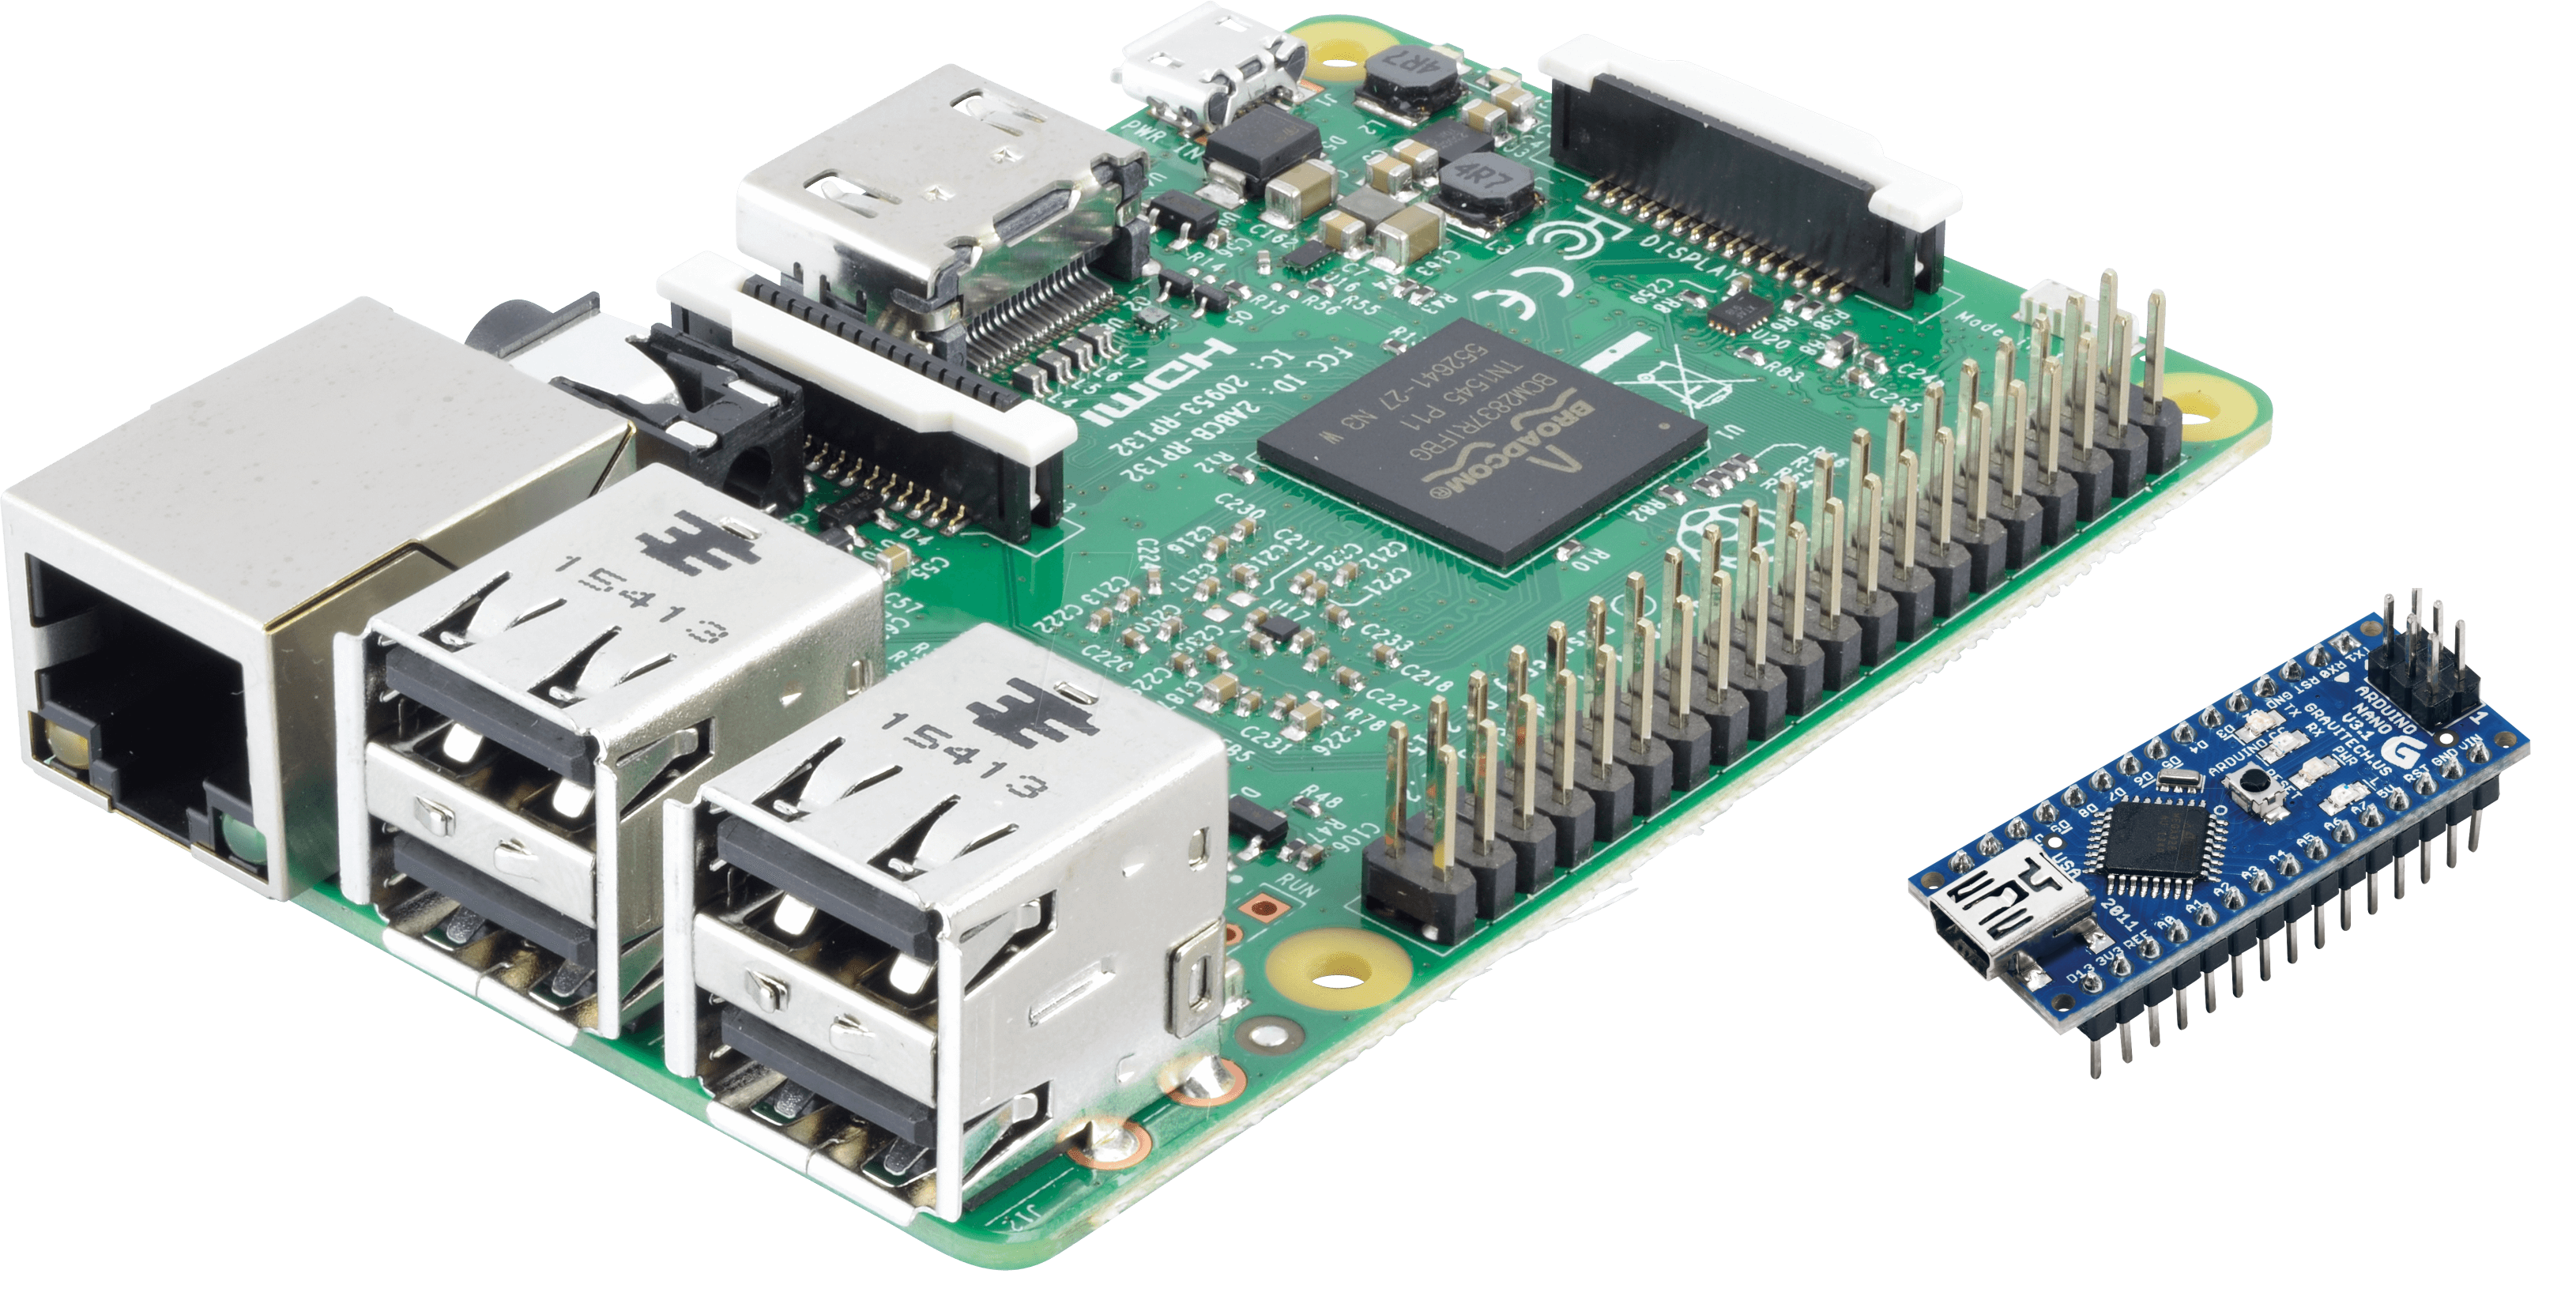
\includegraphics[width=0.7\textwidth]{img/raspArd}
	\caption{Raspberry y Arduino usados}
	\label{fig:RaspArd}
\end{figure}

Como anteriormente hemos comentado, el arduino se encarga de las funciones de control de dirección y velocidad, a continuación mostraremos una imagen del conexionado completo, exceptuando el cable usb que une el arduino y la raspberry.

\begin{figure}[H]
	\centering
	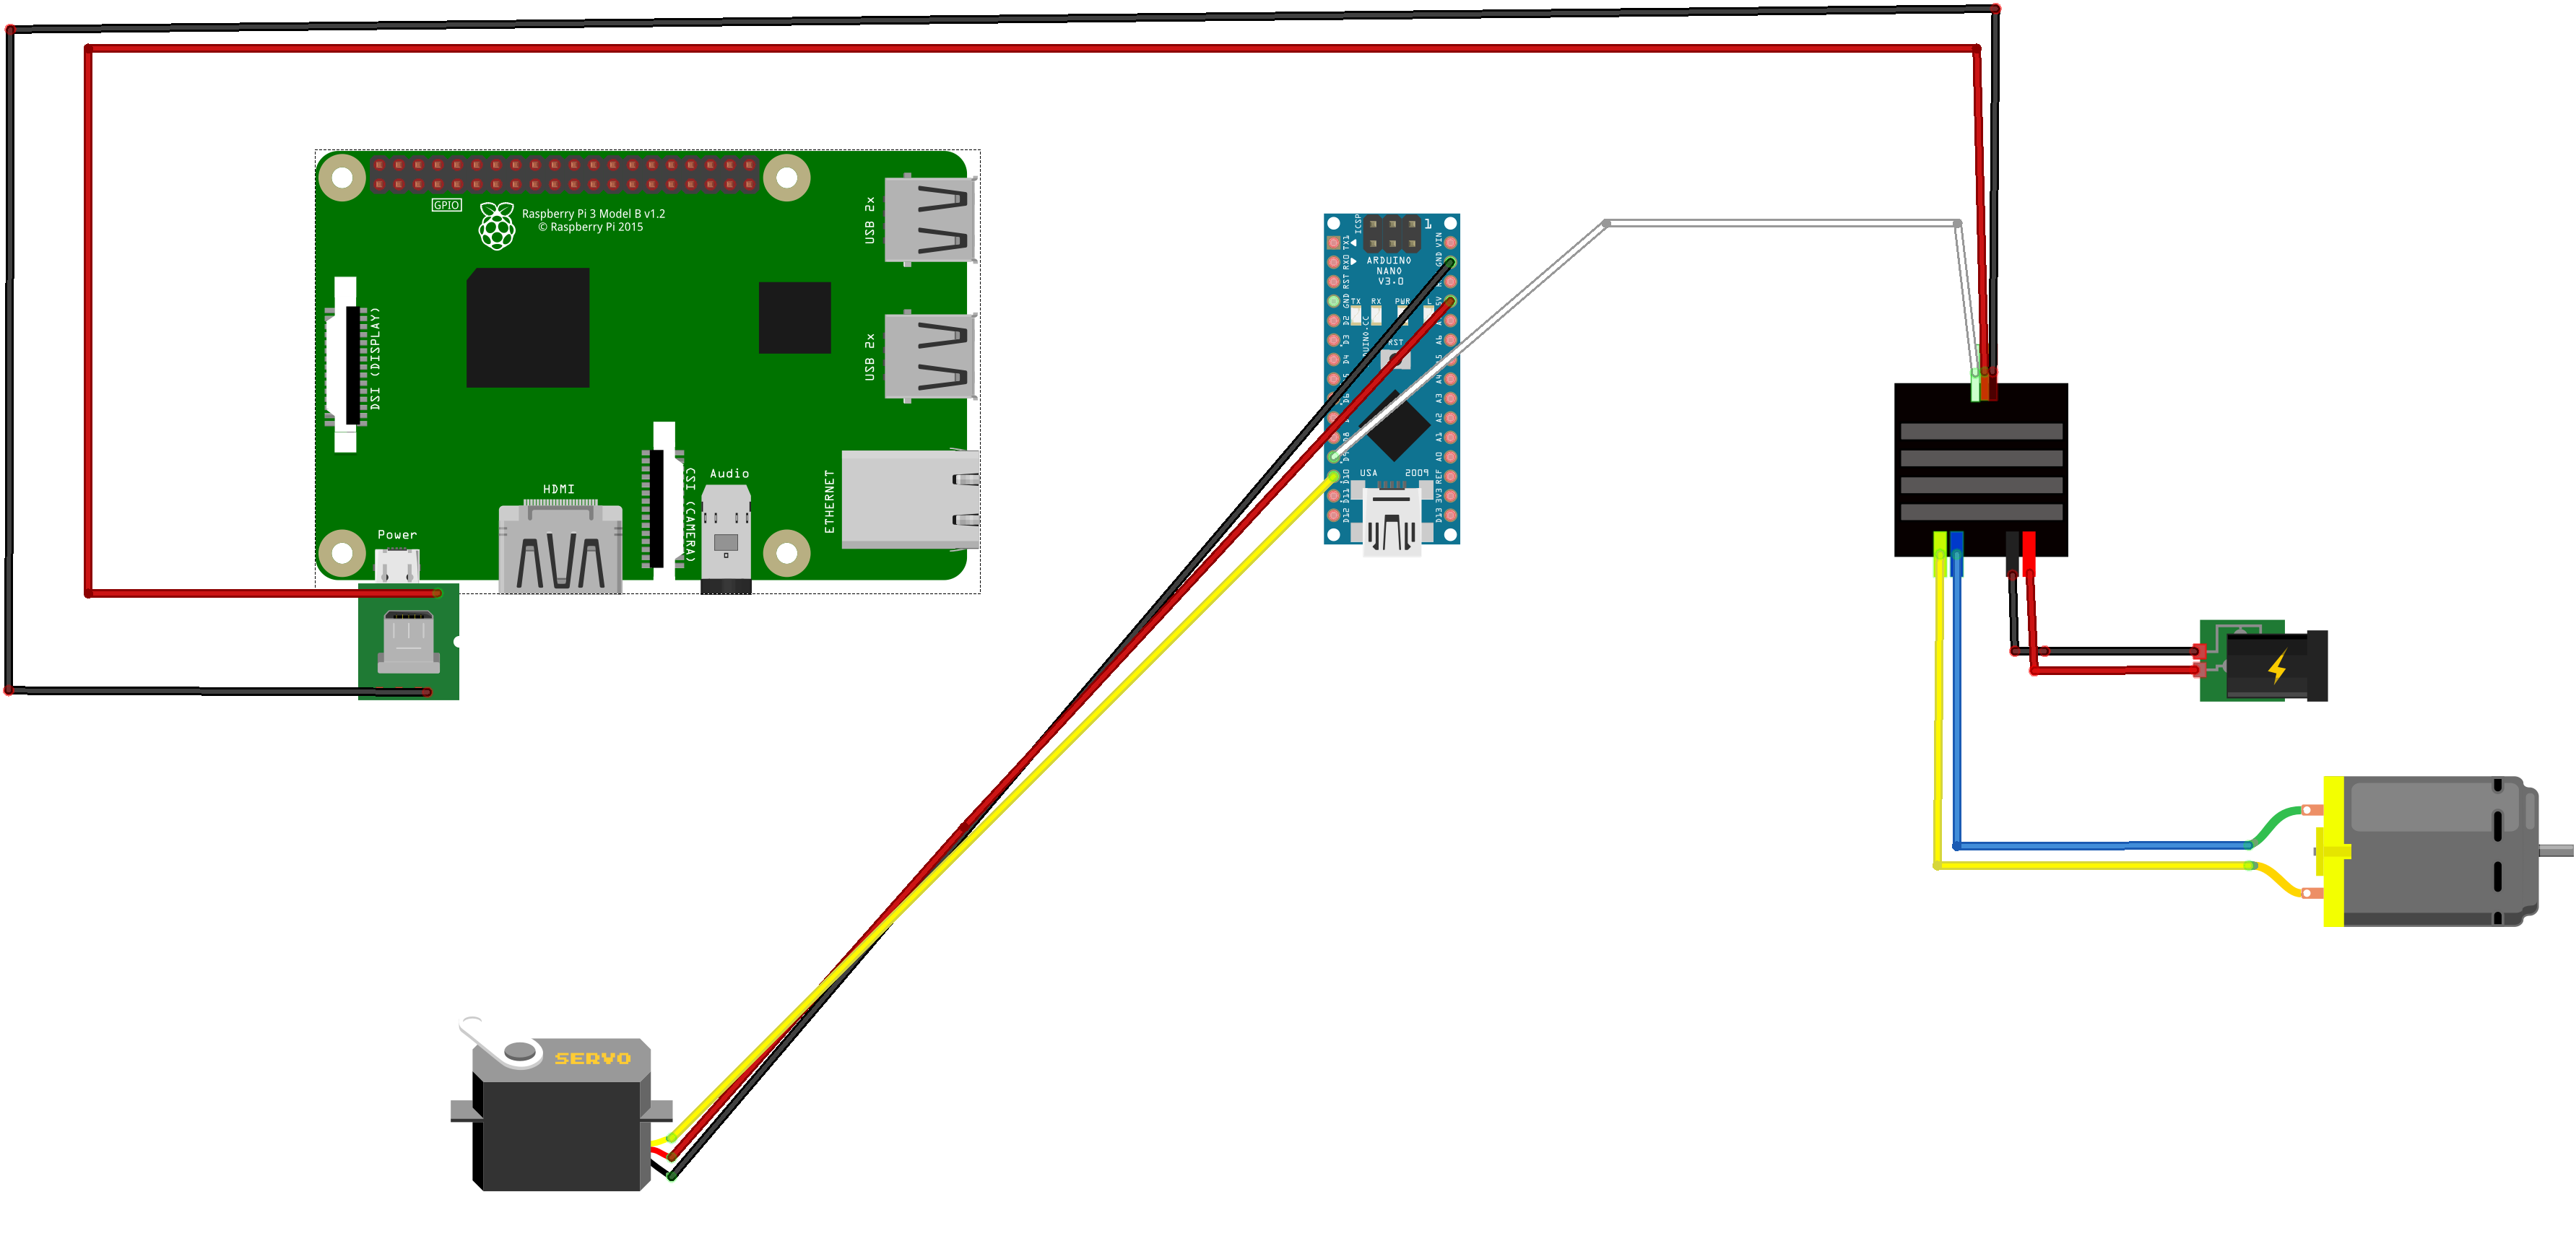
\includegraphics[width=0.9\textwidth]{img/conexionado}
	\caption{Conexionado}
	\label{fig:conexionado}
\end{figure}

Luego de las conexiones entre los distintos dispositivos, añadimos la webcam encargada de enviar las imágenes al sistema receptor. En este caso la webcam es una webcam Usb normal utilizada en un pc cualquiera. Esta se conecta directamente a la raspberry por el puerto USB. 

Para evitar tener tanta cantidad de cables, diseñamos e implementamos una PCB para integrar todas las conexiones y concentrarlo todo en una placa.

\begin{figure}[H]
	\centering
	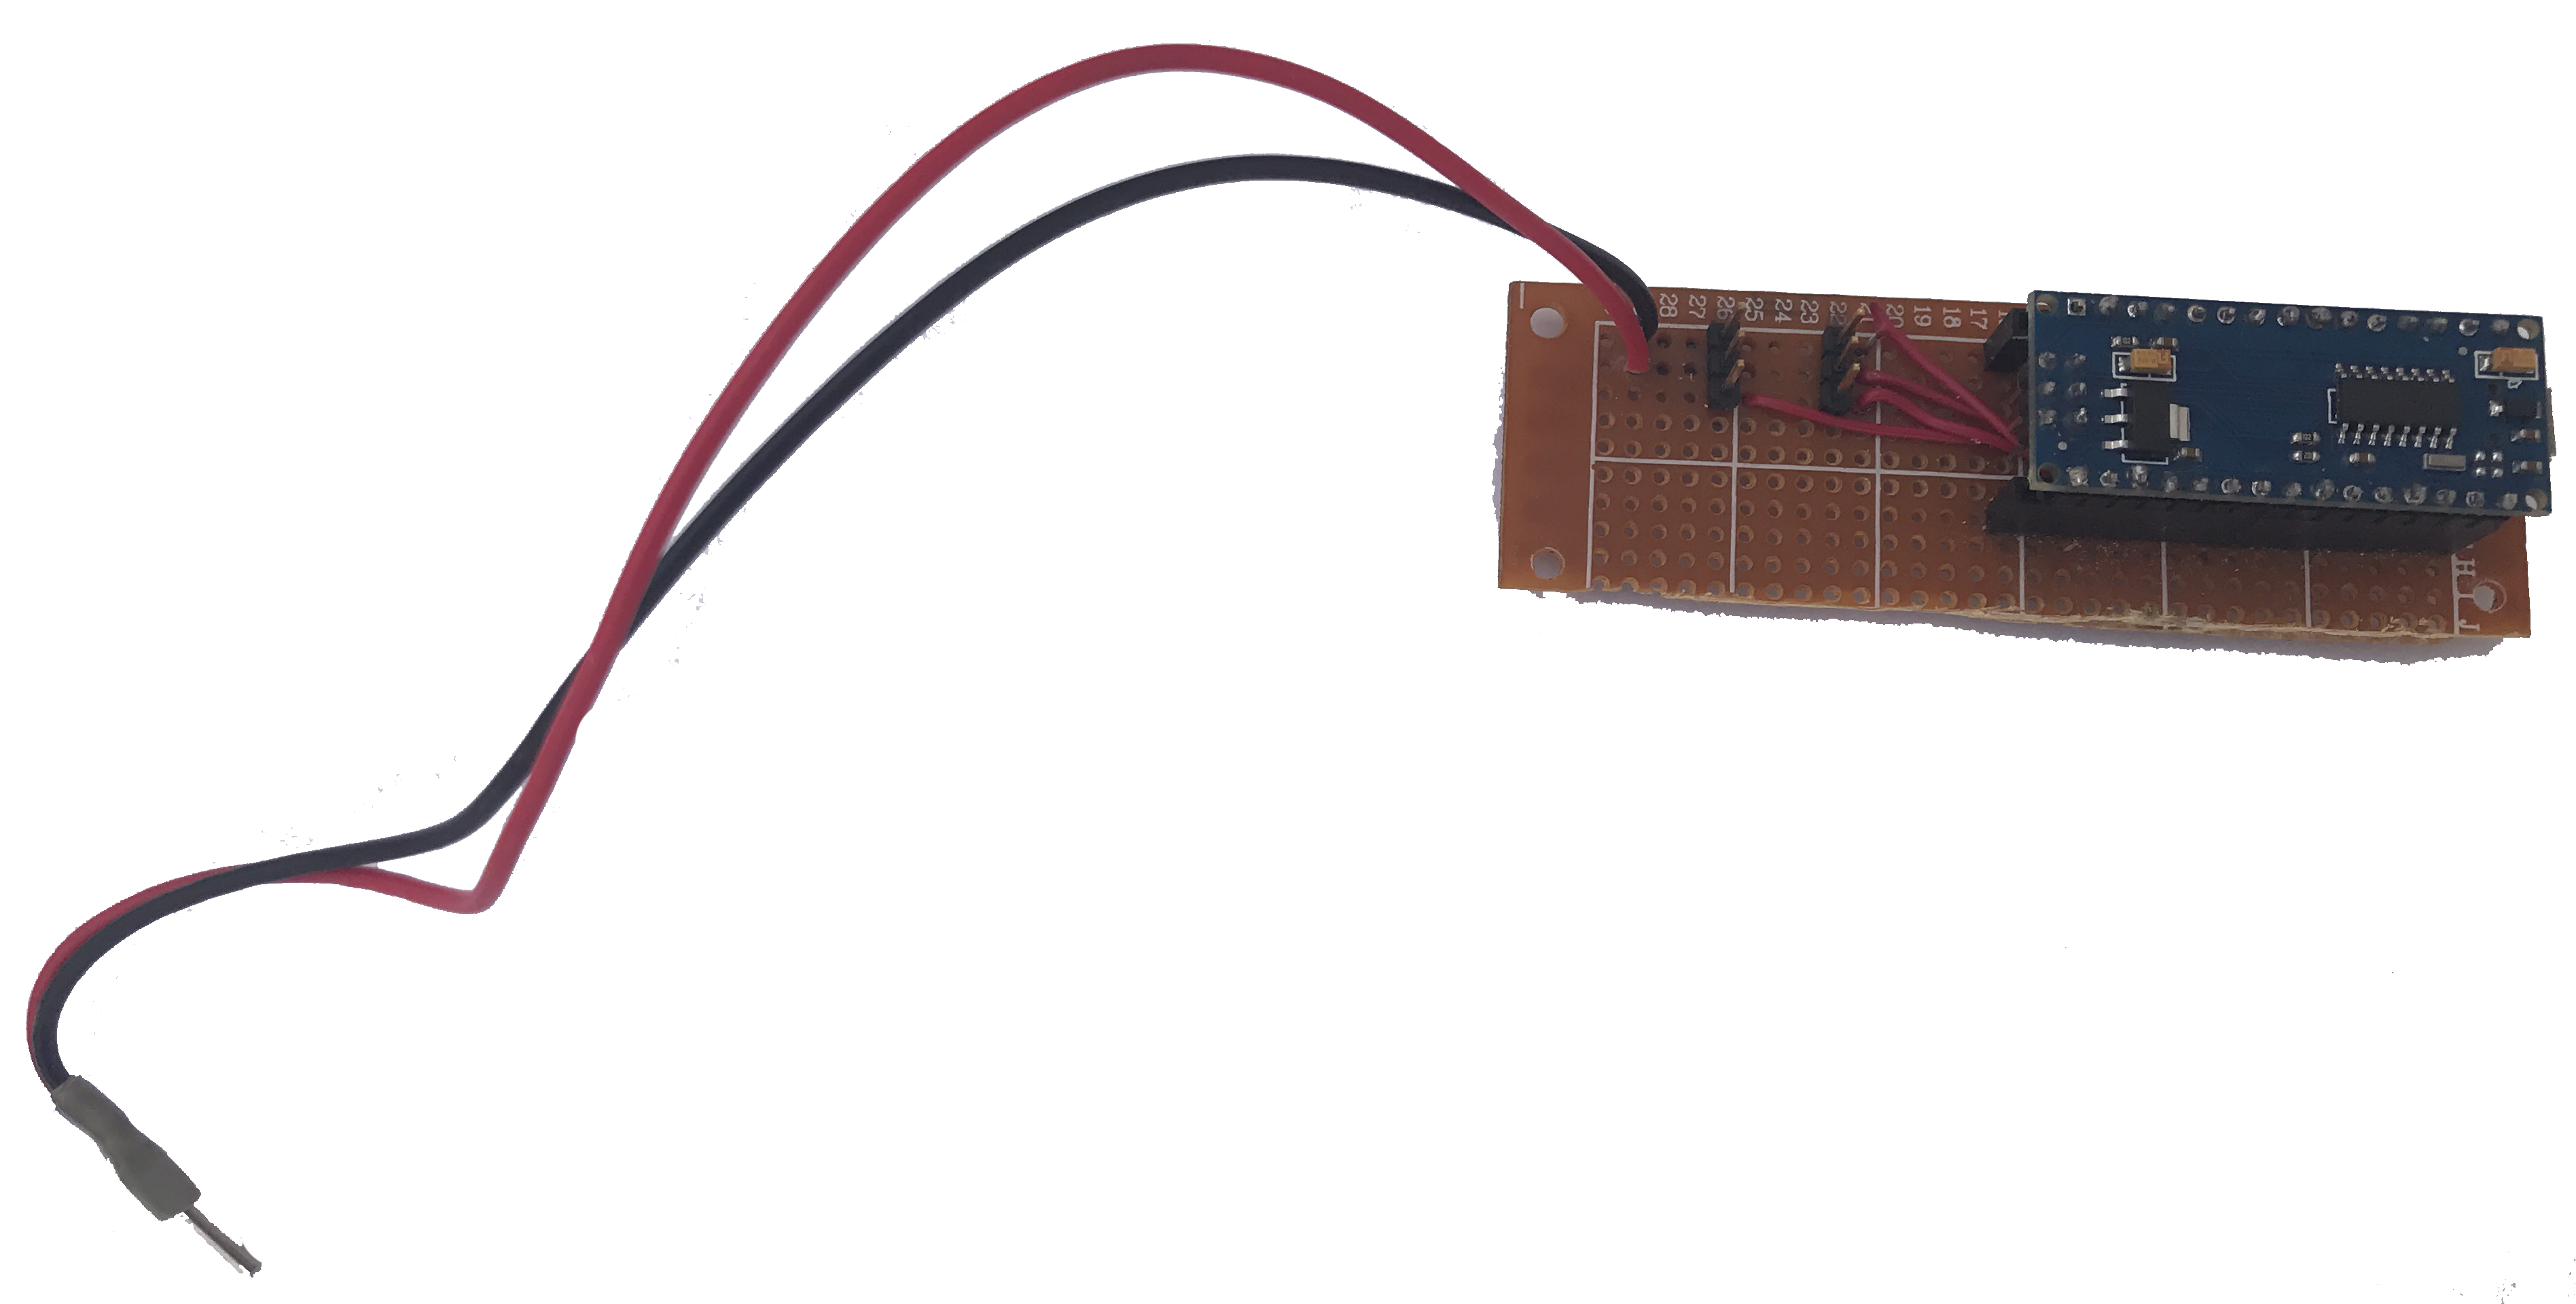
\includegraphics[width=0.7\textwidth]{img/pcb}
	\caption{PCB}
	\label{fig:pcb}
\end{figure}

En un momento determinado del proyecto, ya con las pruebas iniciadas, se detectó un pequeño problema. Este fallo era que al encender el coche, raspberry y arduino necesitan un tiempo prudencial para ponerse en marcha y que funcionen correctamente, pero a simple vista no se sabía cuando ocurría esto. Por tanto se decidió agregarle 3 leds de distintos colores, para saber en que estado se encuentra. Los leds son controlados por los puertos GPIO de la raspberry, en concreto los pines 17, 23 y 24, además se le añadió a cada uno una resistencia para limitar el voltaje que cae en cada led. El diseño del código de color fue el siguiente:

\begin{itemize}
	\item Led rojo: indica que el script python se ha iniciado pero aún no se ha terminado la conexión con arduino y la calibración de los dispositivos.
	\item Led verde: arroja que ya ha acabado el proceso de inicialización y está esperando una conexión entrante.
	\item Led azul: indica que hay una conexión establecida con el servicio de instrucciones (aclarar que el led verde sigue encendido) y por lo tanto se supone que puede haber comunicación entre los pares.
	
\end{itemize}

La imagen que sigue muestra dichos leds y su emplazamiento.

\begin{figure}[H]
	\centering
	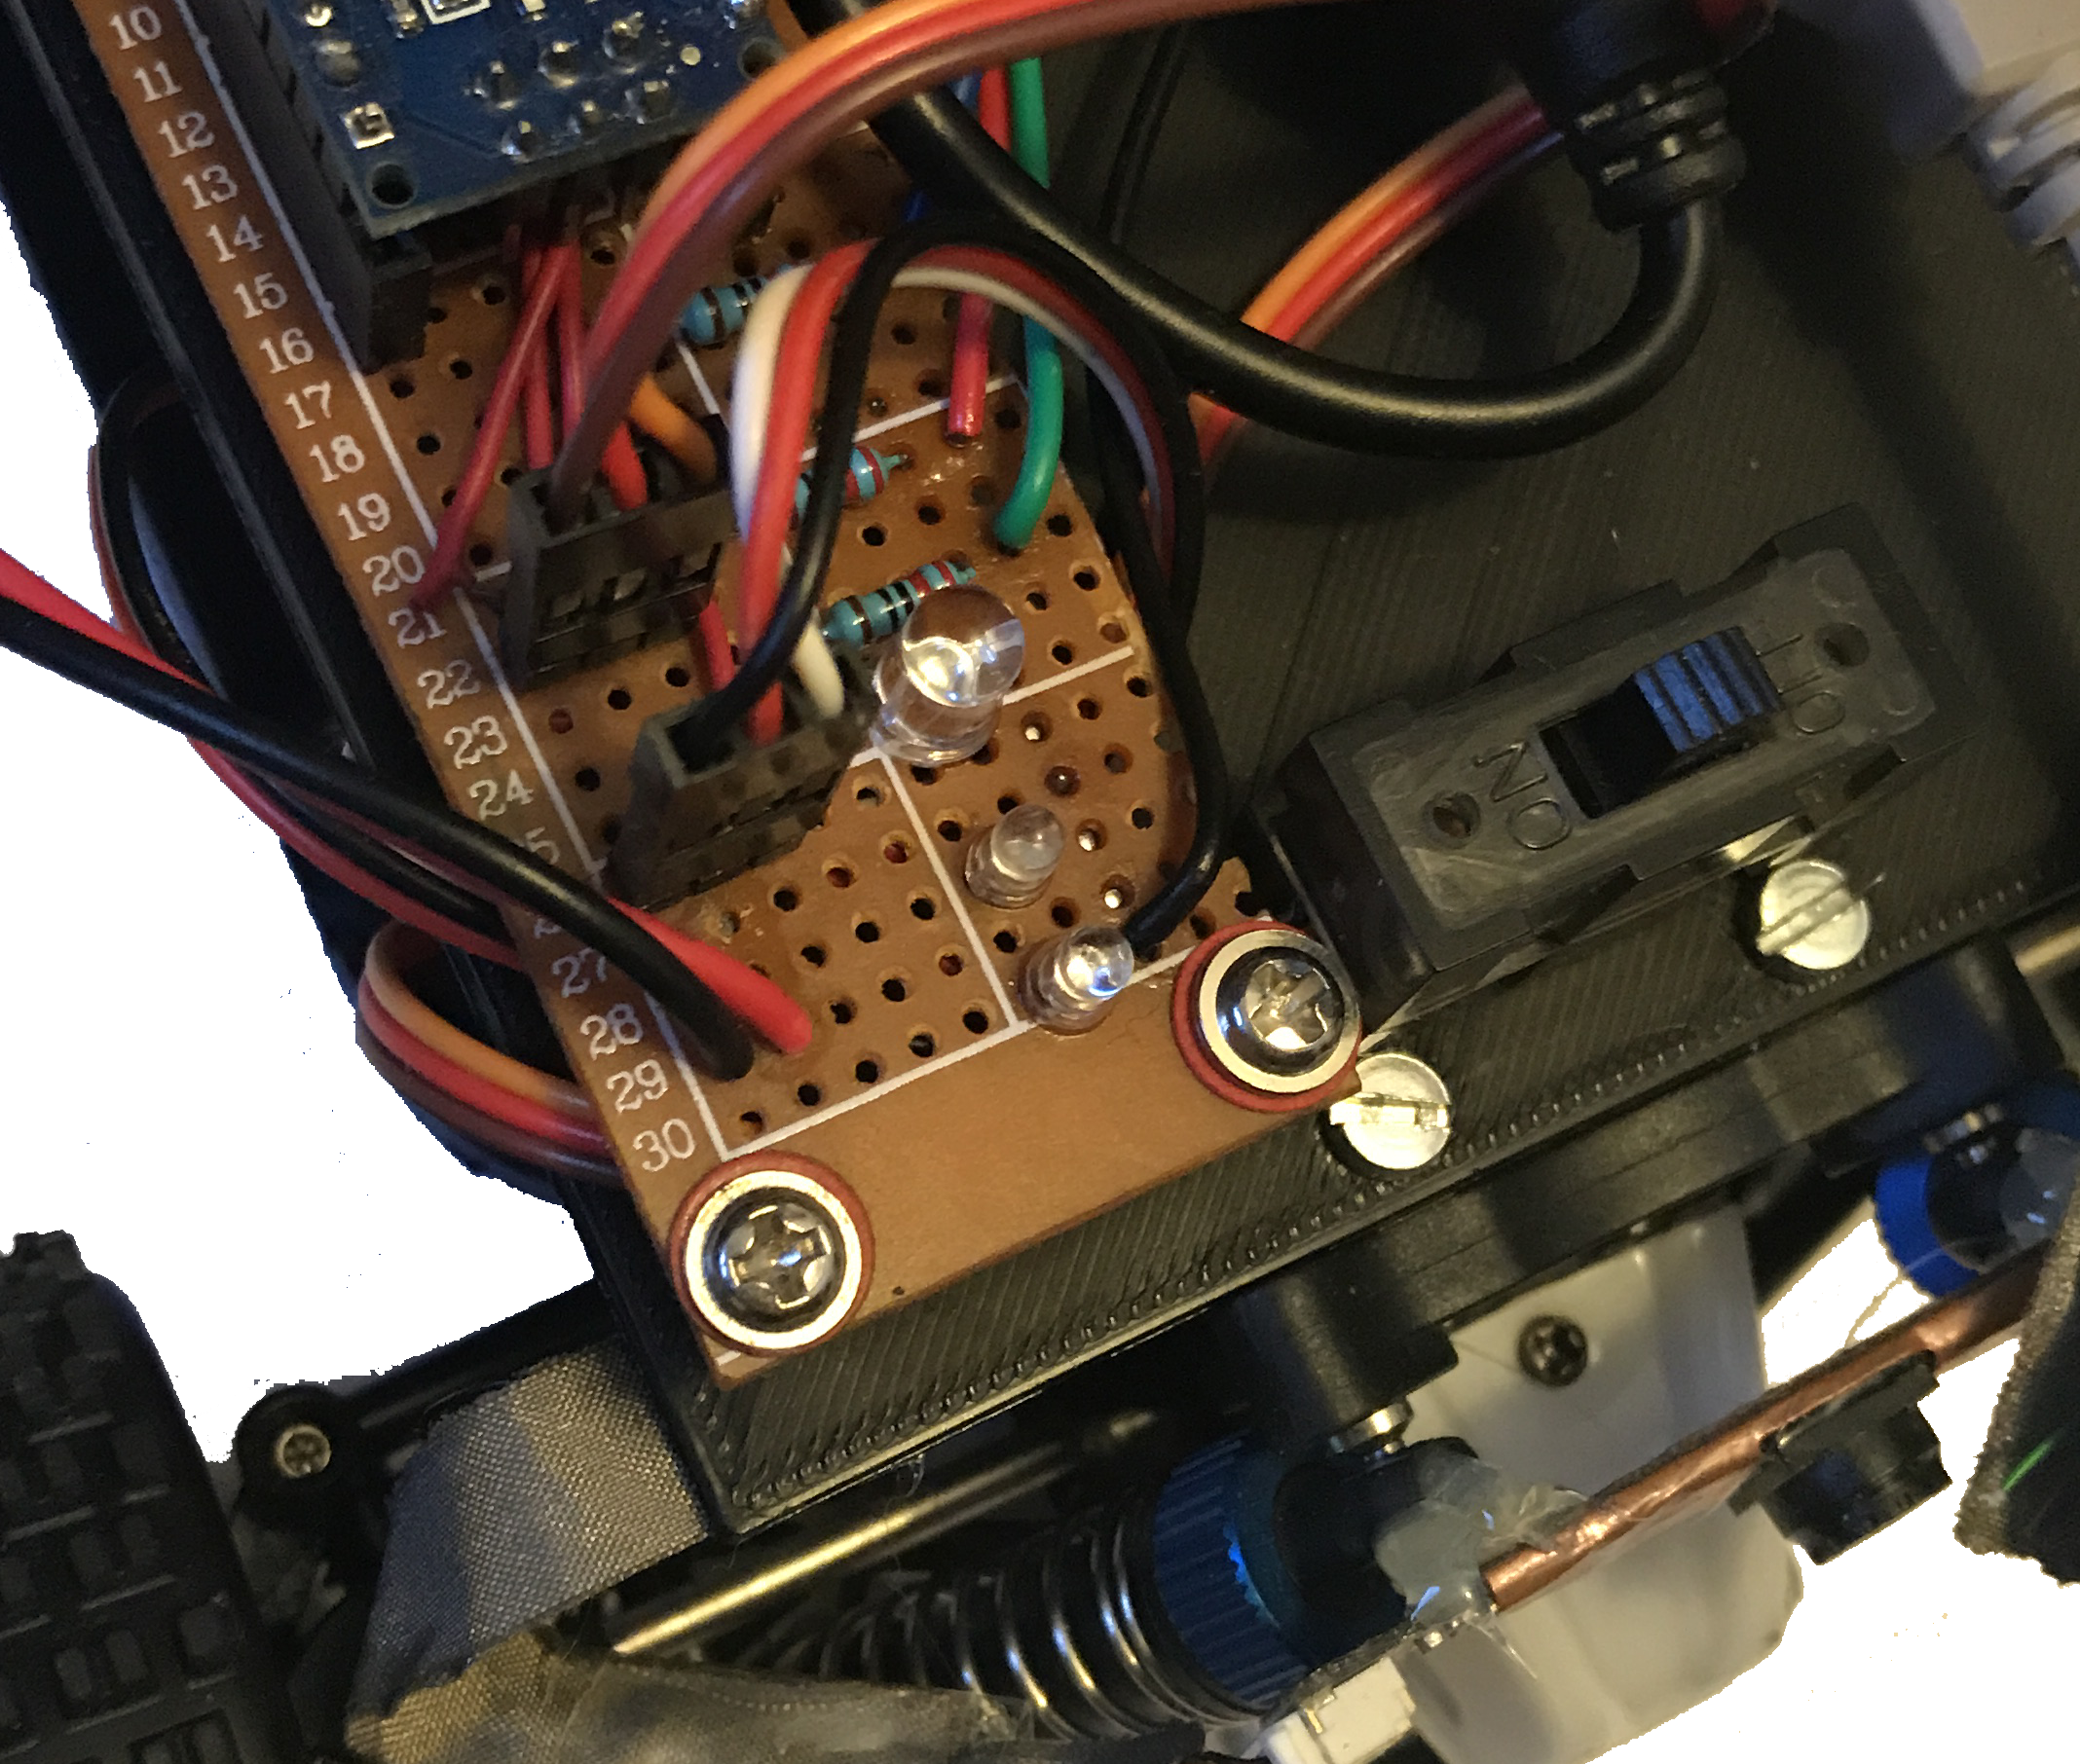
\includegraphics[width=0.7\textwidth]{img/leds}
	\caption{Leds y su emplazamiento}
	\label{fig:leds}
\end{figure}



\begin{figure}[H]
	\centering
	\includegraphics[width=0.7\textwidth]{img/webCamAntigua}
	\caption{WebCam Antigua}
	\label{fig:webcamvieja}
\end{figure}

Después de hablar con una de las personas nombradas en los agradecimientos, llegamos a la conclusión de que esa cámara era demasiado grande y quedaba desorbitada en su emplazamiento. Después de investigar un poco, este cedió una webcam integrada de un portátil, mucho más pequeña e integrable. Tras buscar el datasheet de dicha webcam y usar ingeniería inversa, se procedió a soldar un cable USB. Con esto ya tenemos una webcam mucho más pequeña, instalada como mostraremos a continuación.

\begin{figure}[H]
	\centering
	\includegraphics[width=0.7\textwidth]{img/webcamPortatil}
	\caption{WebCam portátil}
	\label{fig:webcamportatil}
\end{figure}

Llegados a este punto, se hizo necesario buscar la forma de compactar las placas dentro del coche. Para ello se diseñó una placa en la herramienta Tinkercad para ser impresa en 3D. Mostraremos a continuación una captura del diseño de la placa en dicha herramienta.

\begin{figure}[H]
	\centering
	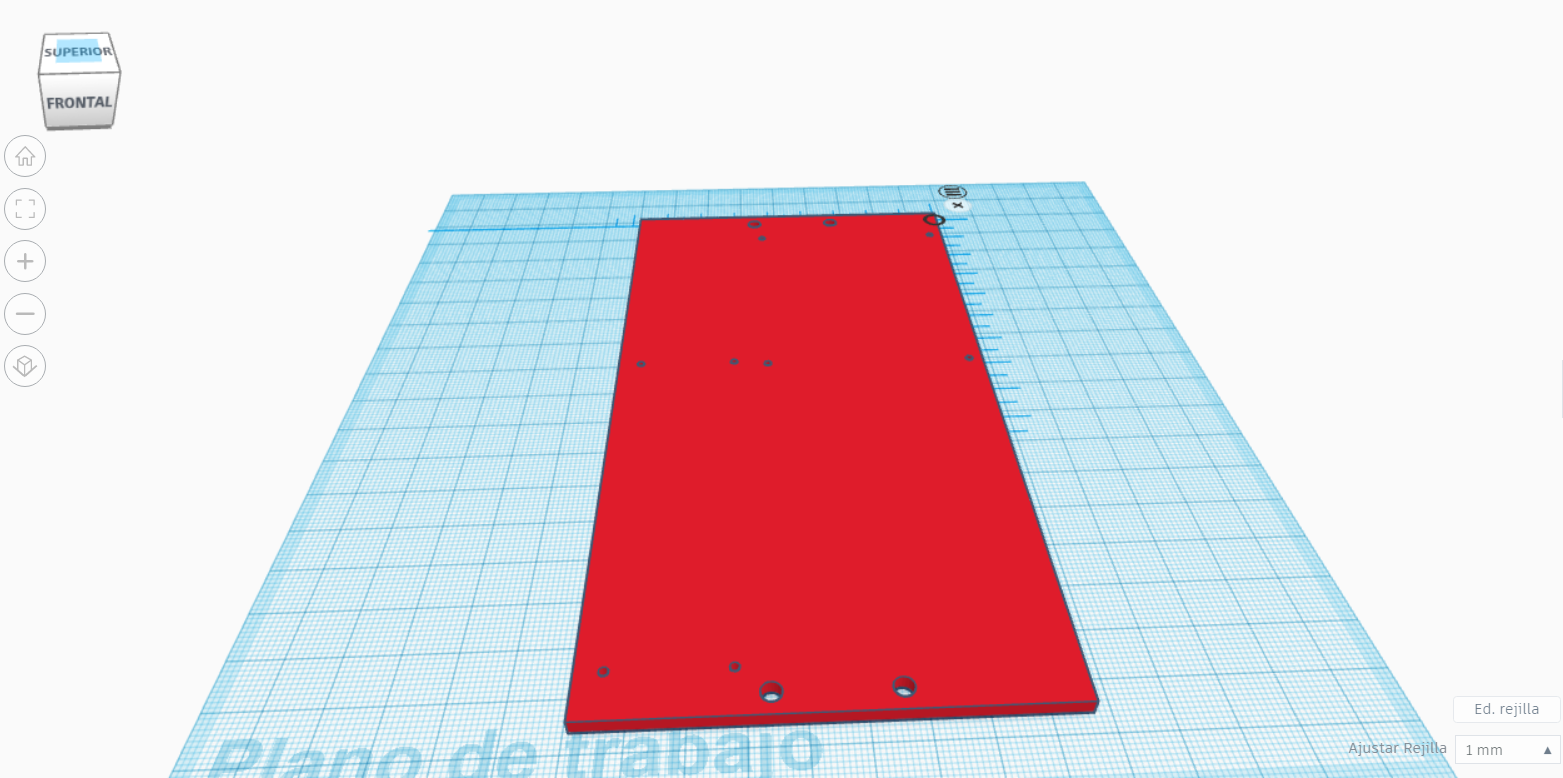
\includegraphics[width=0.9\textwidth]{img/soportePlacas}
	\caption{Placa diseñada 3D para el soporte de la Raspberrry y el Arduino}
	\label{fig:soporteplacas}
\end{figure}

A continuación vemos el resultado de dicho diseño, después de una hora de impresión.

\begin{figure}[H]
	\centering
	\includegraphics[width=0.5\textwidth]{img/soporteImpreso}
	\caption{Placa impresa en 3D}
	\label{fig:soporteplacasimpreso}
\end{figure}

Luego montamos la tornillería necesaria para atornillar la Raspberry Pi y el Arduino.

\begin{figure}[H]
	\centering
	\includegraphics[width=0.5\textwidth]{img/soporteImpresoTuercas}
	\caption{Placa impresa en 3D con la tornillería necesaria}
	\label{fig:soporteplacasimpresotuercas}
\end{figure}

Después de montar la tornillería, añadimos ambos dispositivos, tanto la Raspberry Pi como el Arduino.

\begin{figure}[H]
	\centering
	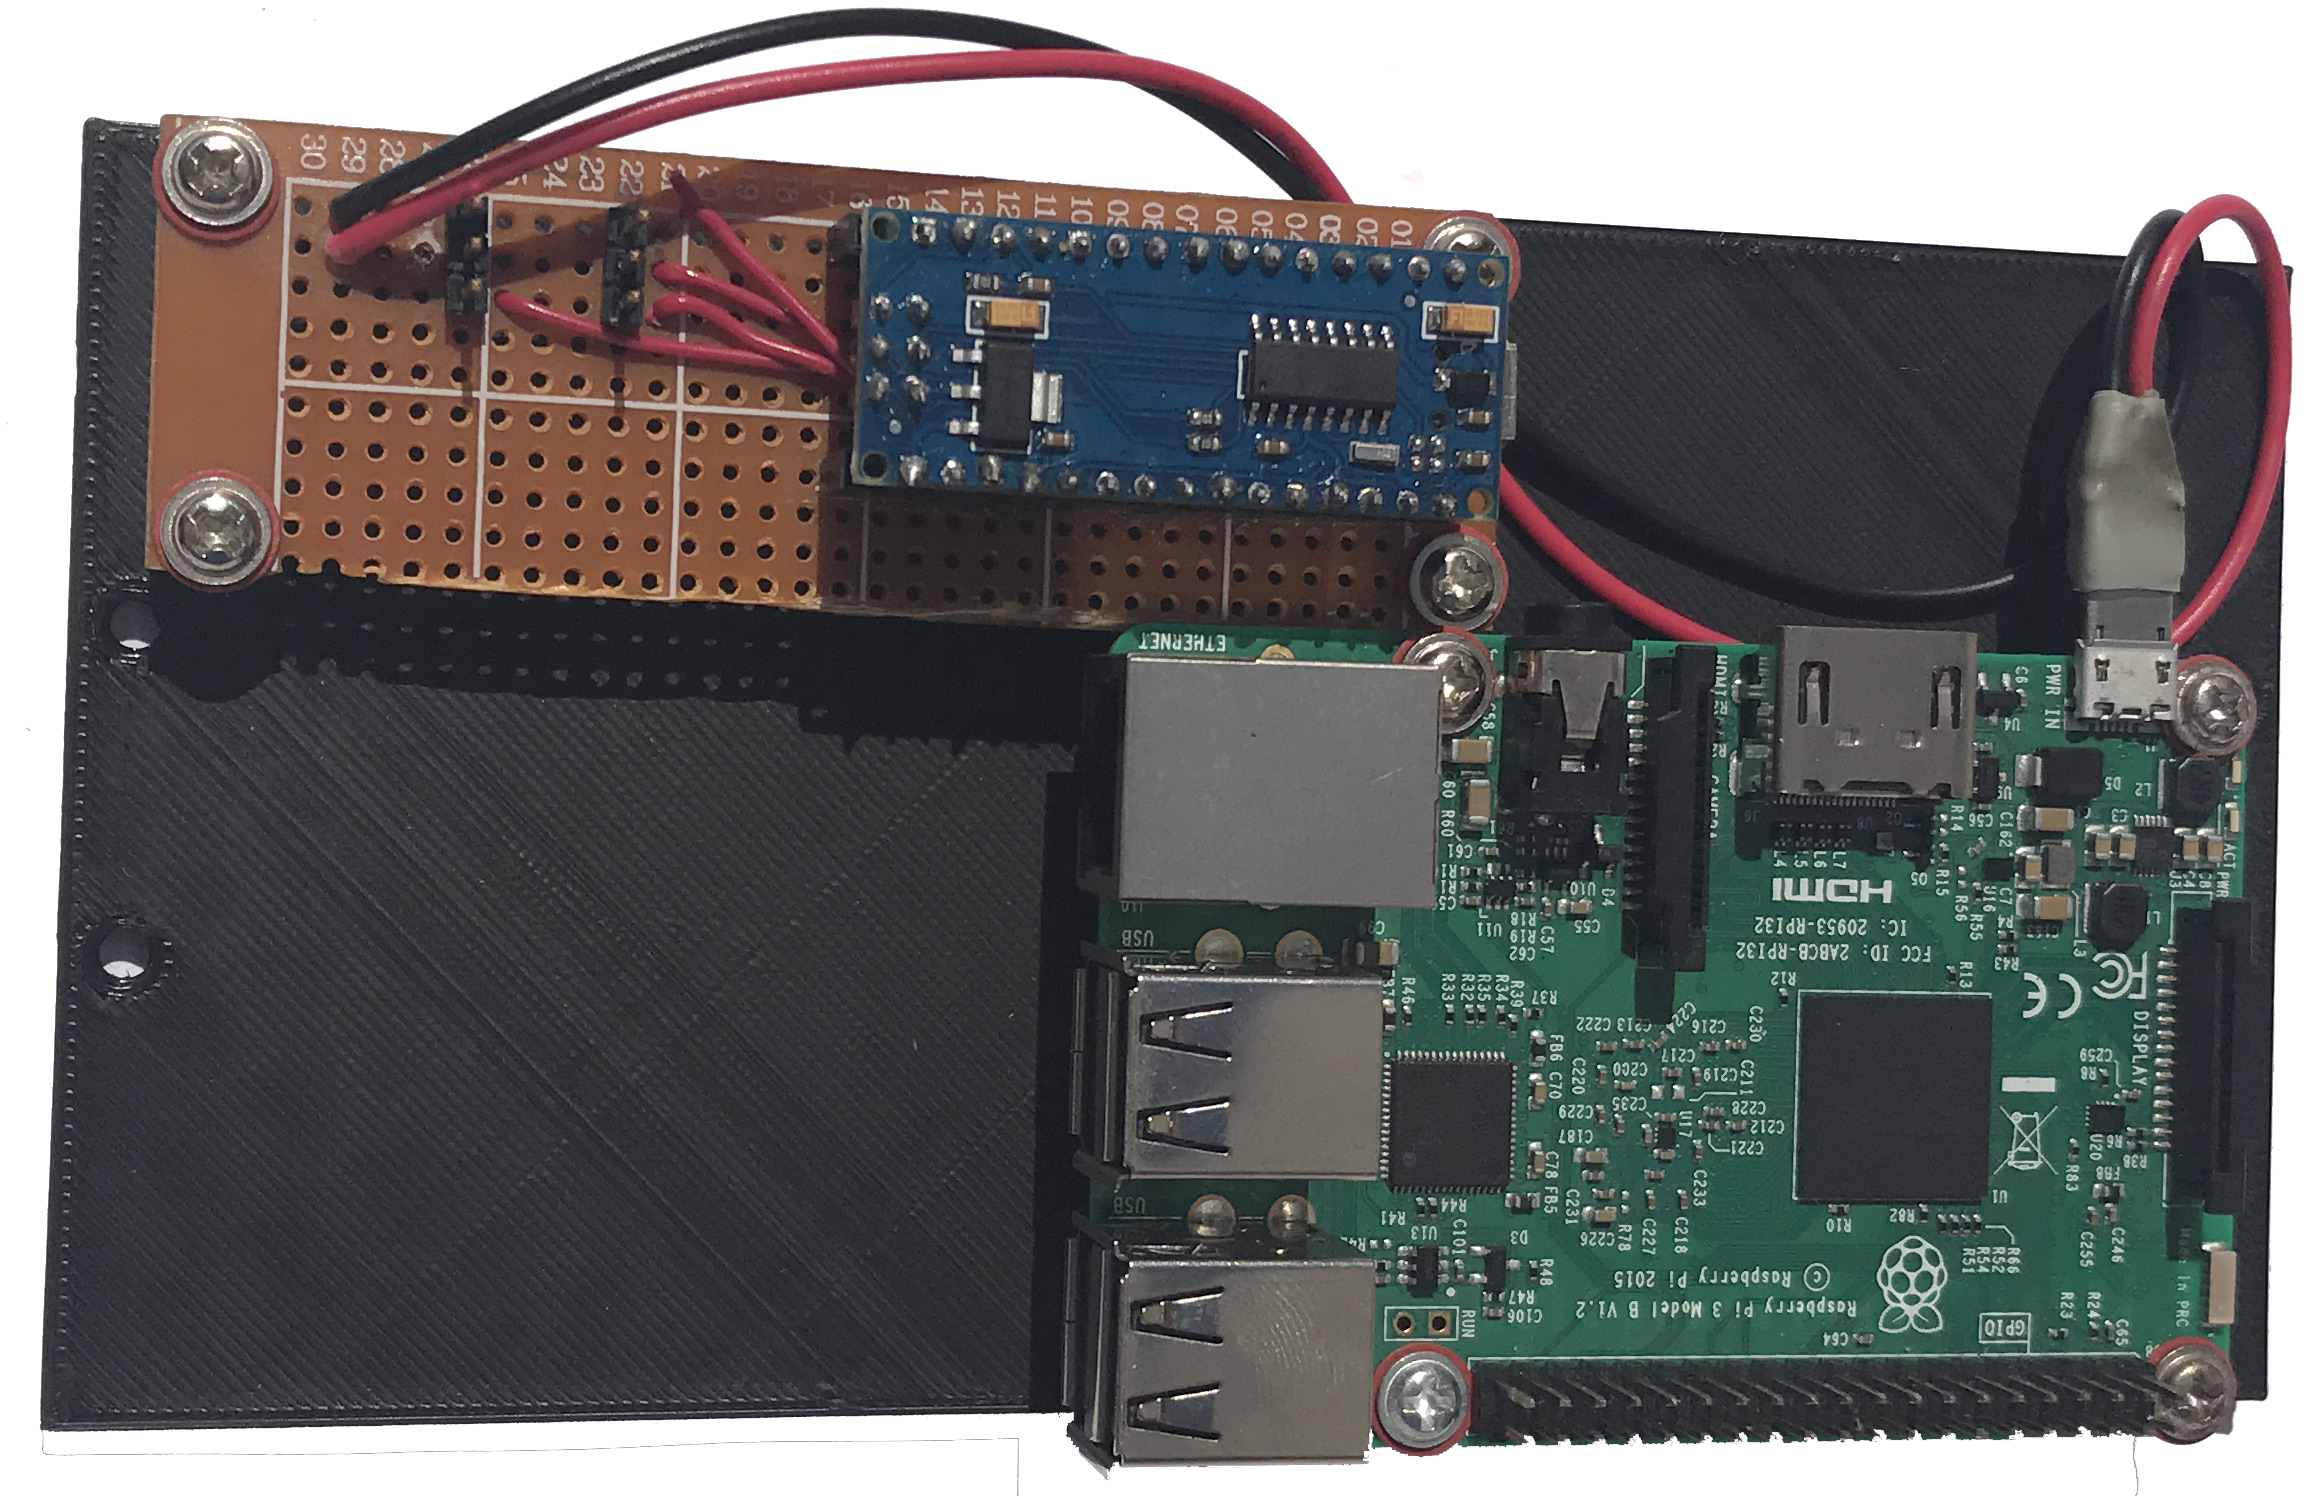
\includegraphics[width=0.7\textwidth]{img/soporteConPlacas}
	\caption{Placa impresa en 3D con los dispositivos montados}
	\label{fig:soporteconplacas}
\end{figure}

En la siguiente imagen mostramos como estaba el prototipo antes de utilizar dicha placa, con muchísimo desorden y con total imposibilidad de probar el prototipo de forma real, ya que cabía la posibilidad de que se desconectara alguna placa y/o hubiera algún daño en estas.

\begin{figure}[H]
	\centering
	\includegraphics[width=0.7\textwidth]{img/cocheConDesorden}
	\caption{Prototipo sin montar la placa de soporte}
	\label{fig:cochesinsoporte}
\end{figure}

A continuación, como la placa estaba diseñada para encajar perfectamente en el coche con cuatro tornillos de anclaje, procedimos a su montaje. Después de acoplar todo en el prototipo, placas, webcam y cableado, quedó algo así, como resultado final.

\begin{figure}[H]
	\centering
	\includegraphics[angle=180,width=0.7\textwidth]{img/resultado}
	\caption{Prototipo resultante con todo montado}
	\label{fig:cochesResultante}
\end{figure}

\item Software


\begin{itemize}
	
	\item Sistema operativo
	
	Como plataforma software donde montar todo el sistema en la Raspberry hemos usado una distribución de linux de Raspberry.org, raspbian jessie lite en concreto , la cual no tiene interfaz gráfica para evitar esa sobrecarga totalmente innecesaria.
	\medskip
	
	\item Conexión inalámbrica
	
	Se han utilizado dos programas para el correcto funcionamiento de la conexión.
	
		\begin{itemize}
			\item hostapd
			\smallskip
			
			Este software nos ha permitido configurar la raspberry para que emita un SSID y cambiar las opciones de este, como puede ser nombre, contraseña, etc.
			\smallskip
			
			\item udhcpd
			\smallskip
			
			udhcpd simplemente es un servidor dhcp que dada la configuracion que hemos introducido se encargará de que al conectar un dispositivo, este reciba una ip adecuada para que el sistema funcione.
			
		\end{itemize}
	\medskip
	\item Arduino
	
	En la parte del hardware comentamos la utilización de un arduino para el control de dirección y tracción/freno. Para su integración, raspberry y arduino se comunican por USB, usándose comunicación serial. Se ha creado un pequeño protocolo de bienvenida entre ambos para asegurar el correcto funcionamiento de la conexión, que a continuación mostraremos.
	
	\begin{figure}[H]
		\centering
		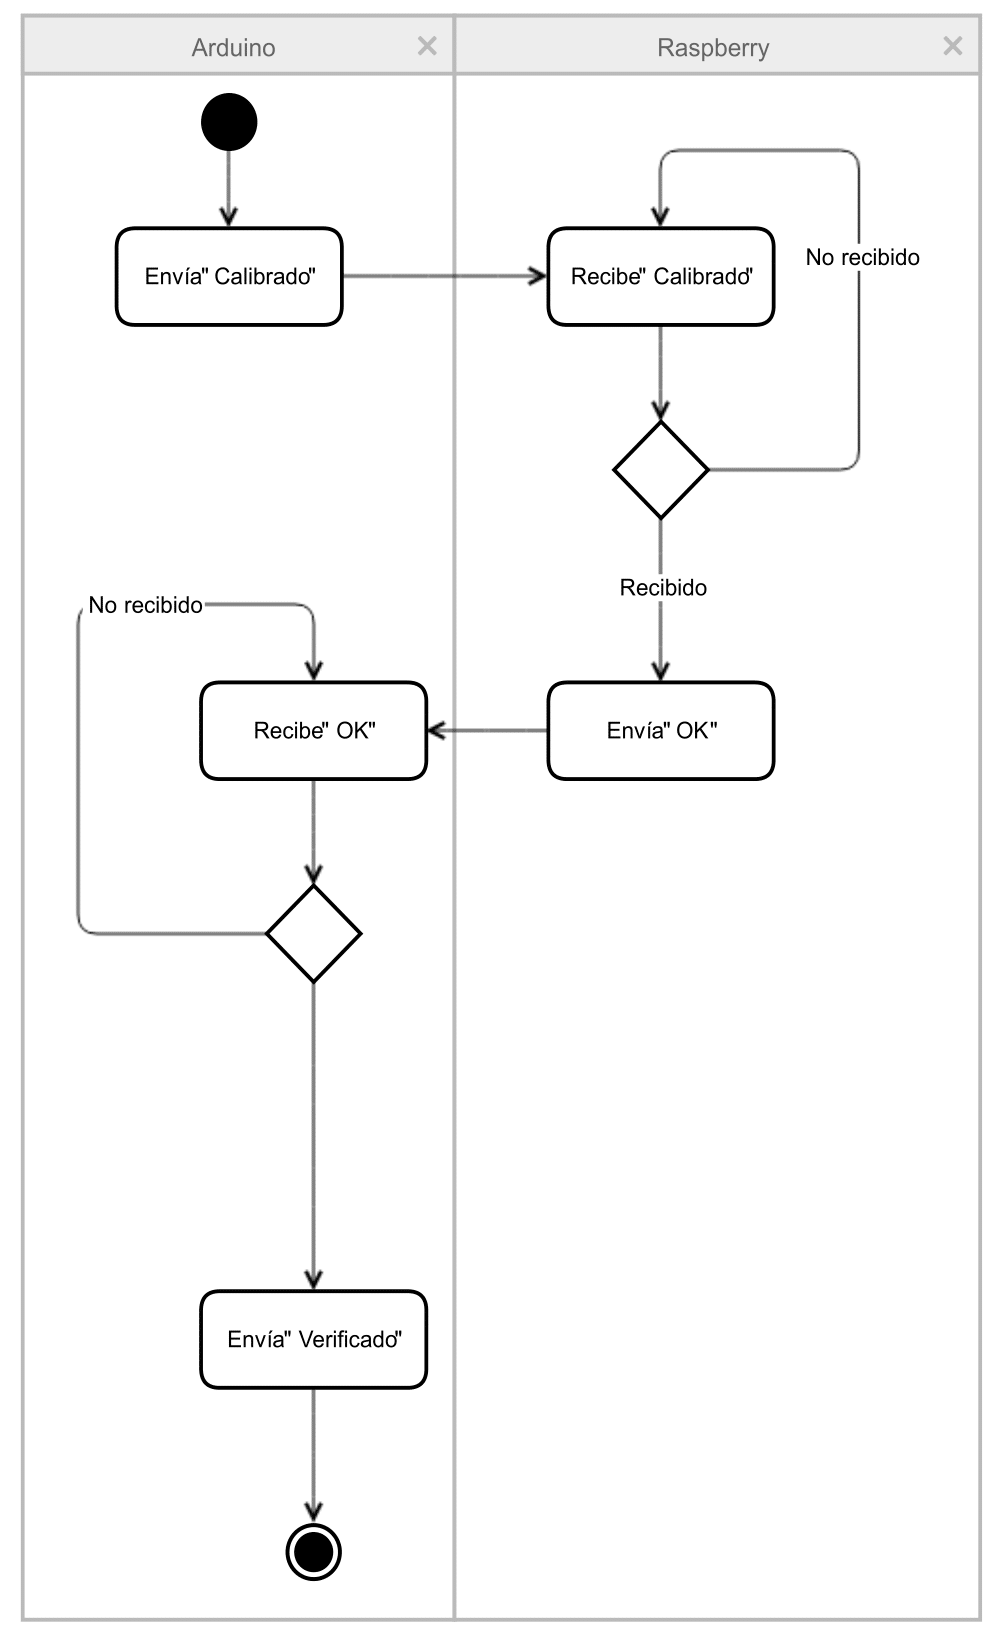
\includegraphics[width=0.7\textwidth]{img/umlComunicacion}
		\caption{UML de la verificación de la comunicación con arduino}
		\label{fig:arduinoVerificacion}
	\end{figure}
	
	Además, se ha creado una codificación entendible por ambos extremos para mandar las instrucciones de lo que el coche debe realizar. Un ejemplo de instrucción sería <<$[$15,115$]$>> y su decodificación:
	\begin{itemize}
		\item $[$ : Carácter de comienzo de instrucción, esto se ha utilizado para reconocer que está comenzando una instrucción.
		\item Aceleración: 15\% 
		\item Dirección: 115º
		\item $]$ : Carácter de terminación de comando, esto se ha utilizado para reconocer el término de una instrucción.
	\end{itemize}
	
	Tras esta explicación cabe aclarar que la primera cifra antes de la coma indica el porcentaje de aceleración del vehículo comprendido entre -100 \% y 100 \%. En segundo lugar aparece la cifra que indica los grados de giro del servo, que teóricamente va desde 0º a 180º, pero que en nuestro caso está limitado a lo que nos deja girar la construcción del mecanismo de dirección que va desde los 65º hasta los 115º.
	

	El arduino recibe dichas instrucciones y las decodifica como hemos descrito. Este respondiendo a una fórmula matemática que se intenta ajustar lo máximo al PWM que soporta el variador y la dirección, sus valores son modificados con una función que maneja los servos dependiendo de los grados a los que queramos posicionarlo y a la aceleración que deseemos imprimir.
	
	\begin{figure}[H]
		\centering
		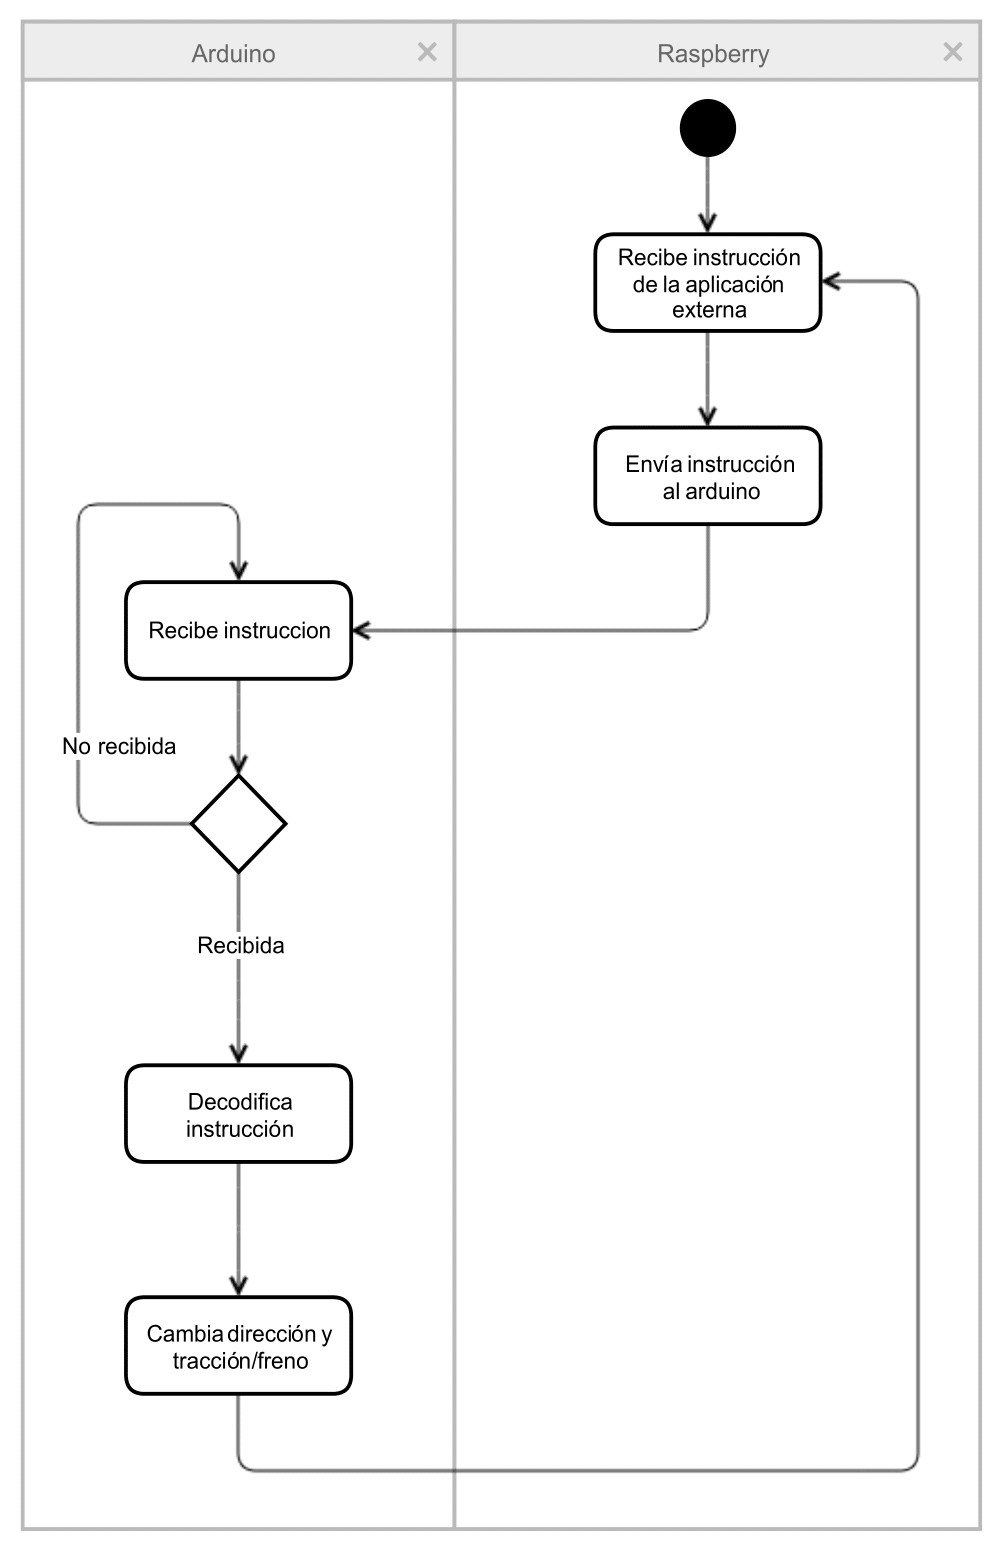
\includegraphics[width=0.7\textwidth]{img/umlCambio}
		\caption{UML de la comunicación del cambio de tracción/freno y dirección}
		\label{fig:arduinoCambios}
	\end{figure}
	
	Al conectar lo primero que el arduino hace es calibrar tanto servo como variador a valores centrales, es decir, el servo a 90º que sería dirección recta, y el variador, mucho más importante porque necesita ser calibrado para su correcto funcionamiento, en un valor central de PWM que indica punto muerto. En este apartado hizo falta mucho tiempo ya que poniendo cualquier valor de PWM el variador no respondía, así que utilizando el método de ensayo y error descubrimos que primeramente hay que calibrarlo pasándole el valor de punto muerto.
	
	\medskip
	
	\item Servicio receptor de comandos
	
	Este es el hilo principal que vertebra a toda la aplicación, escrito en python, en el cual primeramente se crea una variable de la clase arduino, la cual se encarga de verificar internamente la correcta comunicación con este y tiene los métodos necesarios para el envío de comandos al arduino. Aquí el led rojo esta activo, ya que nos indica que no se ha terminado el proceso de inicialización.
	
	En segundo lugar, lanzamos en segundo plano el servicio de streaming de vídeo (mjpg-streamer) que luego comentaremos. Lo hacemos utilizando una conexión a la consola de linux mediante la clase os de python. 
	
	En tercer lugar, creamos el socket de la conexión de datos, la cual utilizaremos para el reconocimiento y procesado de las instrucciones. En este momento apagamos el led rojo y encendemos el verde, que indica que esta listo.
	
	Por último, la aplicación se quedará en bucle infinito esperando que alguien se conecte y si esto ocurre, espera datos de esa conexión hasta que el dispositivo que se ha conectado cierre el diálogo, además al conectarse un cliente, encendemos el led azul para definir que estamos conectados con el cliente. Cada vez que recibe un dato lo procesa y ordena al Arduino que haga los cambios pertinentes. Las instrucciones tienen el mismo formato que las que se envían entre Raspberry y Arduino, con la salvedad de que se incluyen alguna más, como la instrucción ``close'' que sirve para cerrar explícitamente la conexión o la instrucción ``'' que también cierra la conexión y ha sido implementada porque Android al destruir la aplicación, si tiene una conexión activa, manda un paquete con datos vacíos. Cabe decir que la aplicación solo atenderá a una conexión, por simplicidad y porque se supone que solo se conecta un ``controlador'' por llamarlo de alguna manera, no tiene sentido que haya más de un dispositivo que lo controle conectado a la vez. 
	
	Al cerrar la conexión activa, el led azul se apagará indicando que no hay ningún cliente conectado y el script volverá a esperar una nueva conexión entrante.
	
		 SEGUIR LAS MODIFICACIONES
	
	\medskip
	
	\item Servicio streaming vídeo
	
	Para transmitir el vídeo en vivo hemos utilizado mjpg-streamer, un servicio de streaming de vídeo que consume pocos recursos, dado que estamos trabajando en la raspberry, que nos limita mucho. Este además tiene internamente un servidor http para servir las imágenes o vídeos en directo. Esto facilitará mucho el consumo de las imágenes en una posible aplicación de escritorio o en la aplicación Android.
	
	\medskip
	
	\item Procesado de imágenes
	
		En este caso debido a la falta de tiempo, se descartó automatizar el prototipo con procesado de imágenes para solo implementar la detección de personas. La idea era insertar esta parte de código en la Raspberry pero tras probarlo se obtuvo un pésimo resultado en el procesado, ya que la cámara que usamos para el streaming de video es la misma que queremos usar para este motivo. Dicha lentitud es debida a la imposibilidad de usar la cámara en exclusividad. Para ello, lo que se ha hecho es consumir las imágenes directamente del streaming, hecho que nos ralentiza en gran parte. Por contra, ganamos una buena característica y es la posibilidad de que sin modificar el script principal de la aplicación, podemos obtener el control procesando imágenes igualmente pero desde cualquier otro dispositivo, ya sea un PC o un dispositivo móvil.
		
		La manera más fácil que se nos ocurrió para no desaprovechar el trabajo dado la poca cantidad de tiempo disponible a estas alturas, fue procesar las imágenes desde un PC, con lo que ganaríamos en potencia de procesado. También se tuvo en cuenta el poder procesar las imágenes desde la misma aplicación Android ya diseñada, pero por facilidad y falta de tiempo, nos decantamos por la primera. Para ello hemos usado el mismo principio, descargar la imagen del streaming y procesarla luego. 
		
		Entrando en detalles del propio script
		
		En la imagen que sigue detallaremos con un diagrama de estados el funcionamiento de dicho programa.
		
		\begin{figure}[H]
			\centering
			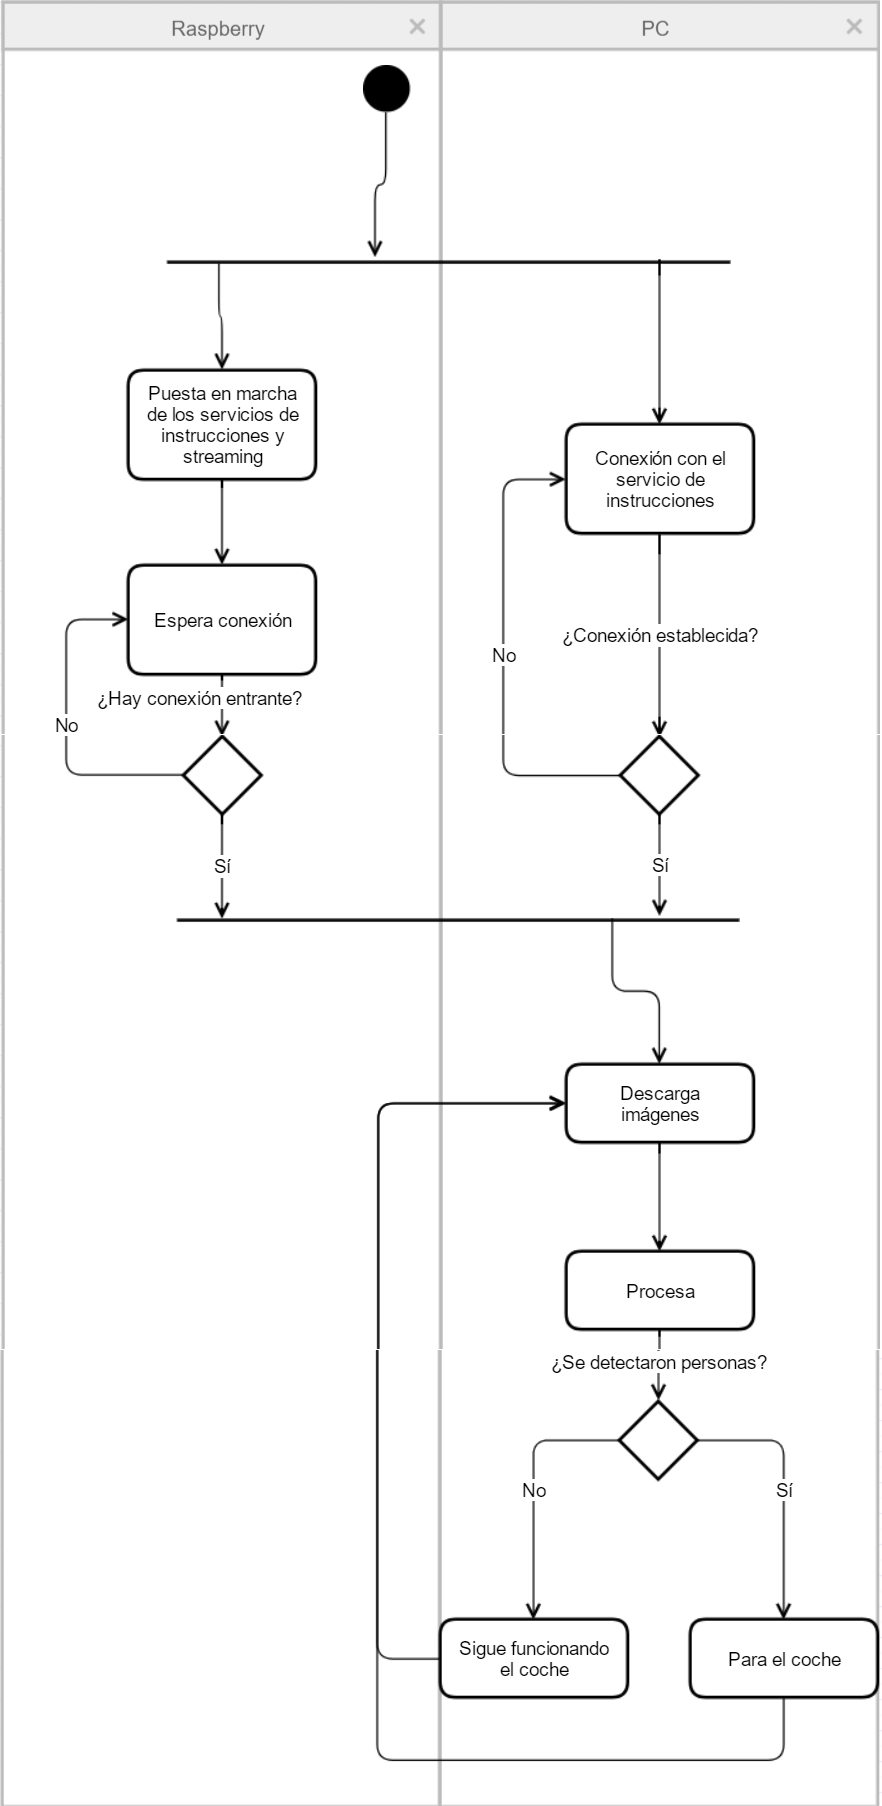
\includegraphics[width=0.7\textwidth]{img/procesadoUML}
			\caption{UML del procesado de imágenes}
			\label{fig:procesadoUML}
		\end{figure}
		
	
		\cite{OpenCV}

	\medskip

	\item Aplicación android
	
	La aplicación Android esta basada en una app ya existente de código libre, obtenida de un repositorio en Bitbucket, llamada simpleMJPGView \cite{simpleMJPG}, que en principio, simplemente se dedica a consumir las imágenes que el coche emite con el protocolo MJPG. Tras obtener el código y añadirlo a Android Studio comenzamos las modificaciones necesarias para adaptarlo a nuestros requisitos. En primer lugar, se ejecutó la parte más importante de la aplicación, la conexión con el servicio de instrucciones del coche. Se tomó de referencia la IP que tenemos en las opciones de la aplicación. Tras ello la aplicación lanza un hilo en el que se hace una conexión TCP hacia el puerto 10000 de nuestra raspberry. Al conectar ya tenemos disponible el canal de comunicación de instrucciones. Luego se abre la conexión HTTP al puerto 8080 de nuestra raspberry para obtener el stream de imágenes para representarlas en la aplicación. 
	
	Una vez todas las conexiones están activas se inicializa el acelerómetro para escuchar el sensor y mandar sus datos a la dirección del coche. Para evitar que el tráfico de instrucciones sea muy alto debido a las continuas lecturas del acelerómetro, se ha discretizado el valor de este a la parte entera, ya que así obviamos diferencias pequeñas de dirección y ruidos. Además solo se vuelve a mandar un comando si es distinto al anterior para evitar enviar varios comandos con el mismo valor. En cuanto al control de aceleración, ya sabemos que el prototipo tiene una velocidad alta, con lo que desde la aplicación solo permitimos el 50 \%  de la potencia disponible. Al igual que en la dirección hemos usado la misma táctica en cuanto a no repetir instrucciones ya enviadas. En el acelerador sí permitimos que el control actúe con toda su precisión porque da pasos de 1 unidad, algo asumible en cuanto a diferencia de aceleración y de tráfico generado.
	
	A continuación mostraremos unas capturas de la aplicación ejecutada en una tablet Samsung Galaxy Tab 3 7":
	
	\begin{figure}[H]
		\centering
		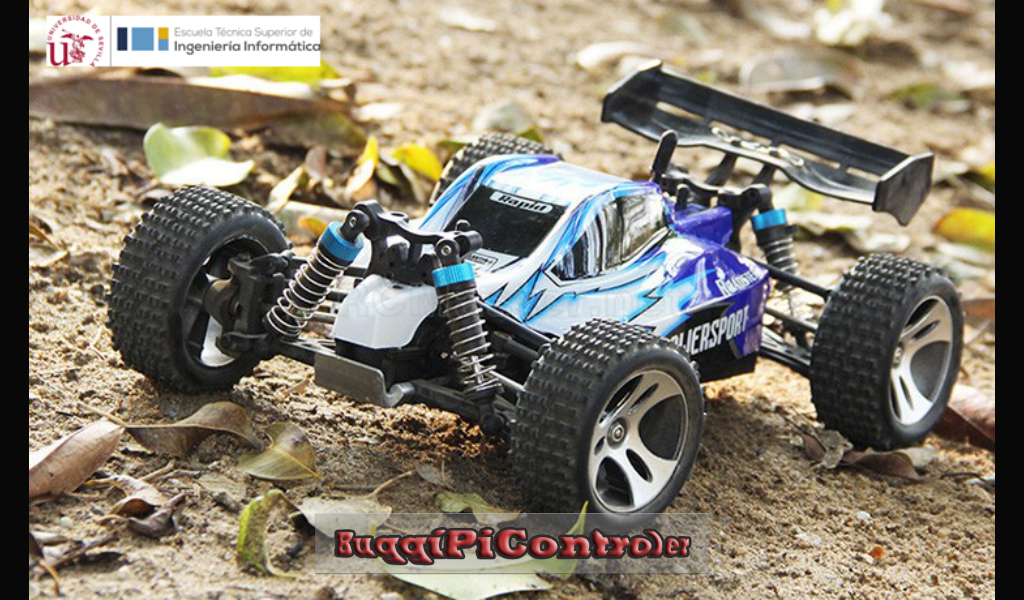
\includegraphics[width=0.7\textwidth]{img/inicio}
		\caption{Captura de la pantalla de inicio de la aplicación}
		\label{fig:capturaInicio}
	\end{figure}

	\begin{figure}[H]
		\centering
		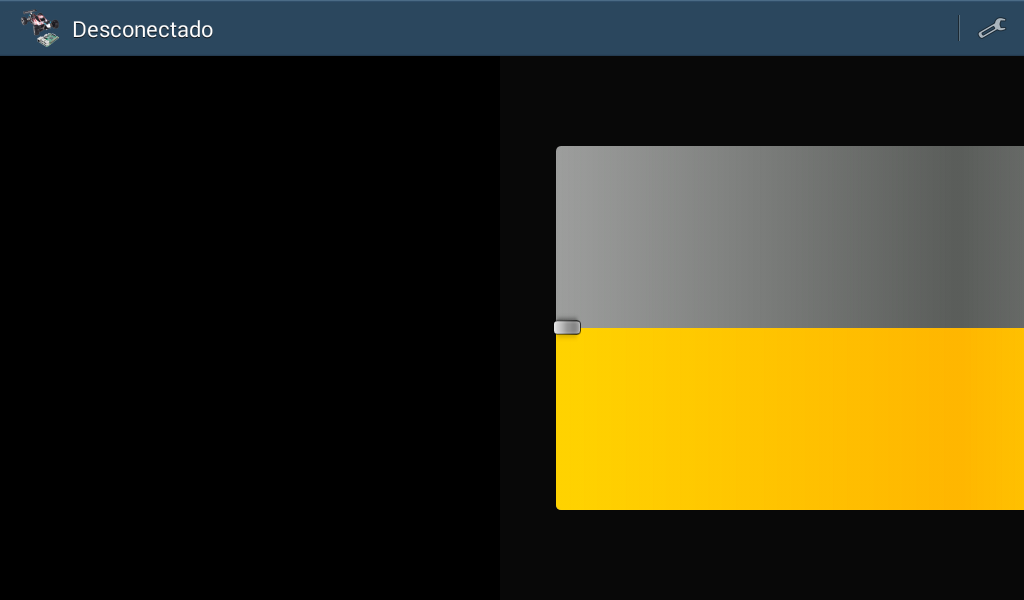
\includegraphics[width=0.7\textwidth]{img/sin_conexion}
		\caption{Captura de la pantalla principal de la aplicación sin conexión}
		\label{fig:capturaSinConexion}
	\end{figure}

	\begin{figure}[H]
		\centering
		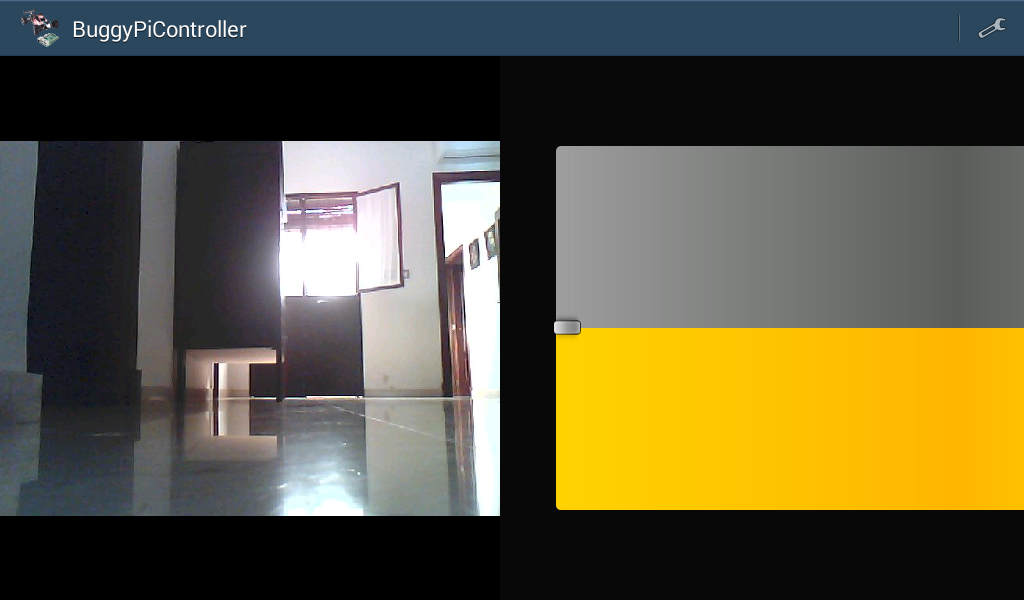
\includegraphics[width=0.7\textwidth]{img/conectado}
		\caption{Captura de la pantalla principal de la aplicación funcionando}
		\label{fig:capturaConConexion}
	\end{figure}
	
	\begin{figure}[H]
		\centering
		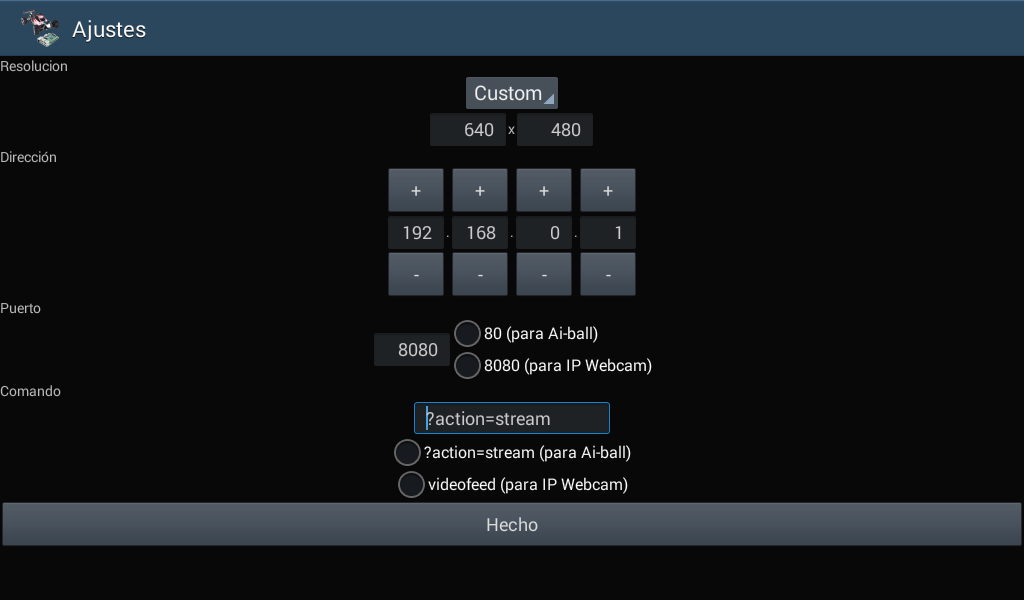
\includegraphics[width=0.7\textwidth]{img/opciones}
		\caption{Captura de la pantalla de opciones de la aplicación}
		\label{fig:capturaOpciones}
	\end{figure}
	
	
	\medskip
	
\end{itemize}
\end{itemize}


\section{Pruebas del sistema} 

Las pruebas realizadas del sistema han sido muy diversas, ya que en cada paso del diseño del software y hardware correspondiente se han sucedido todo tipo de test por partes para cerciorar el correcto funcionamiento de las modificaciones. A continuación pasaremos a describir las más importantes:

\begin{itemize}
	\item Arduino:
	
		Las primeras pruebas que se realizaron en el proyecto fueron bastante simples y se hicieron en esta parte del proyecto. Se empezó simplemente probando el control de servo y variador, una simple prueba de como responden estos ante el control del arduino. Esta se realizó lanzando unas instrucciones concisas y prefijadas para comprobar el correcto funcionamiento de las piezas descritas.
		
		Después de comprobar que todo era posible y funcionaba correctamente se realizó el software en arduino que recibía las instrucciones, este las decodificaba y actuaba en consecuencia. En este paso, para verificar el correcto funcionamiento, conectábamos el arduino al puerto USB del pc y desde el IDE de arduino entrabamos al monitor del puerto serie. A continuación mandabamos los comandos pertinentes para ejecutar el protocolo de bienvenida perfectamente. En cuanto estaba preparado para recibir instrucciones se lanzaba una serie de órdenes predefinidas y con ciertos errores, para cerciorar que en todo momento realizaba lo que esperábamos. 
		
	\item Raspberry:
	
		Antes de empezar con el servidor que debe ser el principal servicio que preste la raspberry, había que configurar el wifi. Para ello, utilizamos otra microSd para no modificar el sistema donde se estaba desarrollando. En esta nueva microSd se realizaron las pruebas pertinentes para las configuraciones deseadas de la conexión wifi y por ende, la del servidor dhcp.
	
		En cuanto al sistema python implementado en la raspberry hay dos claras pruebas que se han realizado.
		
		En primer lugar se implementó la conexión por USB con el arduino. Con lo cual se lanzaron una serie de pruebas en las cuales se enviaban una batería de comandos desde el código python por serial al arduino y que este respondiera tal cual se esperaba de él.
		
		Como segunda prueba, se comprobó la parte de la conexión para las instrucciones. En este caso, primeramente se hizo un cliente también en python que se conectara al servicio, para verificar la correcta recepción de los comandos. Luego ya se hizo la misma prueba pero ya conectando desde una primera versión de la aplicación android.
		
		Como última prueba, se unió el servicio de escucha de instrucciones y la conexión con el arduino. Ya una vez unido, se volvieron a repetir las pruebas anteriores. Desde un script python se le enviaba una batería de instrucciones y solo cabía esperar que el coche hiciera las indicaciones. Tras el éxito, se hizo lo mismo pero desde android, con una primera versión de la aplicación android.
		
	
	
	\item Webcam:
	
		Igual que en el apartado anterior, usamos la microSd de pruebas para probar los distintos sistemas de streamer. Se probaron un script python con opencv para la obtención de imágenes, que fue descartado por el alto consumo de recursos. Luego se hicieron todas las pruebas con el streamer ahora utilizado, MJPEG-Streamer. En este se probó en primera instancia tomar imágenes e irlas guardando en un directorio pero también era bastante pesado. Así que la última configuración fue la más acertada. Este streamer tiene la opción de emitir directamente a un servidor HTTP. Con esto lo lanzamos y comprobamos desde cualquier navegador cual era el resultado y si la velocidad de transmisión era aceptable.
		
		Luego ya integrado con el script principal de los servicios, probamos la aplicación SimpleMJPEG de android, para consumir las imágenes y comprobar si era fluida las imágenes.
	
	\item Aplicación:
	
		Como anteriormente comentamos la aplicación se ha probado en dos partes. En primer lugar la parte de sensor de aceleracion de la tablet y el slider, todo ello con la conexión de instrucciones. Para ello se usó una aplicación con solo esta parte y se usó durante unos 20 min para comprobar la respuesta del vehículo.
		
		En segundo lugar se comprobó la parte del consumo de imágenes. Para ello solo hubo que encender el servicio y hacer unas pruebas de si las imágenes se recibian y si es aceptable el flujo que nos ofrece.
		
		Por último se completó la aplicación y con ambas partes y se puso a prueba si había demasiado retardo al añadir ambas cosas al canal de la comunicación.
	
	\item Funcionamiento completo:
	
		
	
\end{itemize}


\chapter{BLOQUE 3: PLANIFICACIÓN DEL PROYECTO}
\section{Planificación temporal inicial} 
A continuación detallaremos una planificación temporal a priori:

\begin{figure}[H]
  \centering
    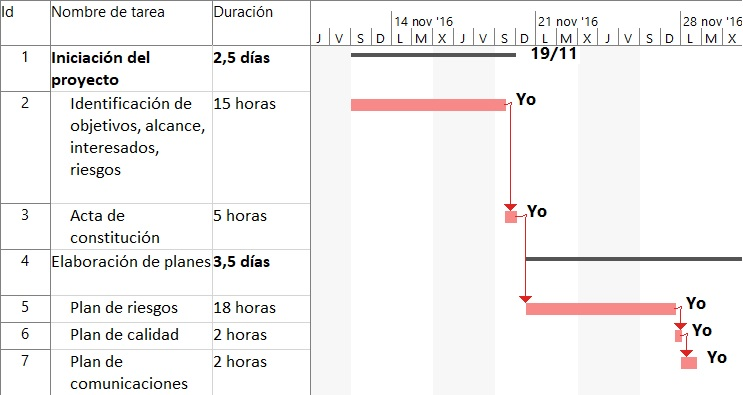
\includegraphics[angle=270,width=0.5\textwidth]{img/ganttInicial}
  \caption{Diagrama de Gantt Inicial}
  \label{fig:ganttInicial}
\end{figure}

\begin{figure}[H]
	\centering
	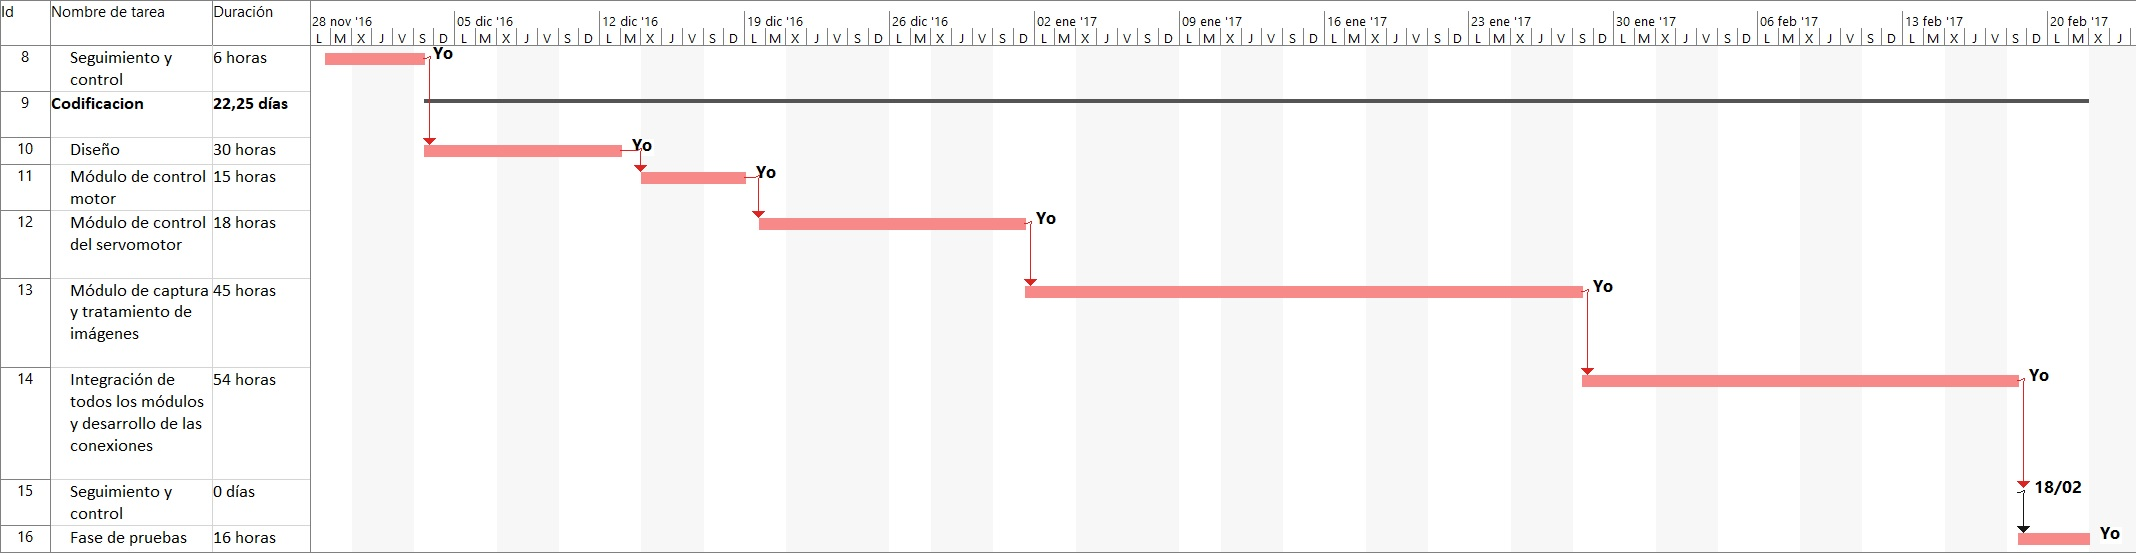
\includegraphics[angle=270,width=0.45\textwidth]{img/ganttInicial_2}
	\caption{Diagrama de Gantt Inicial 2}
	\label{fig:ganttInicial2}
\end{figure}

\begin{figure}[H]
	\centering
	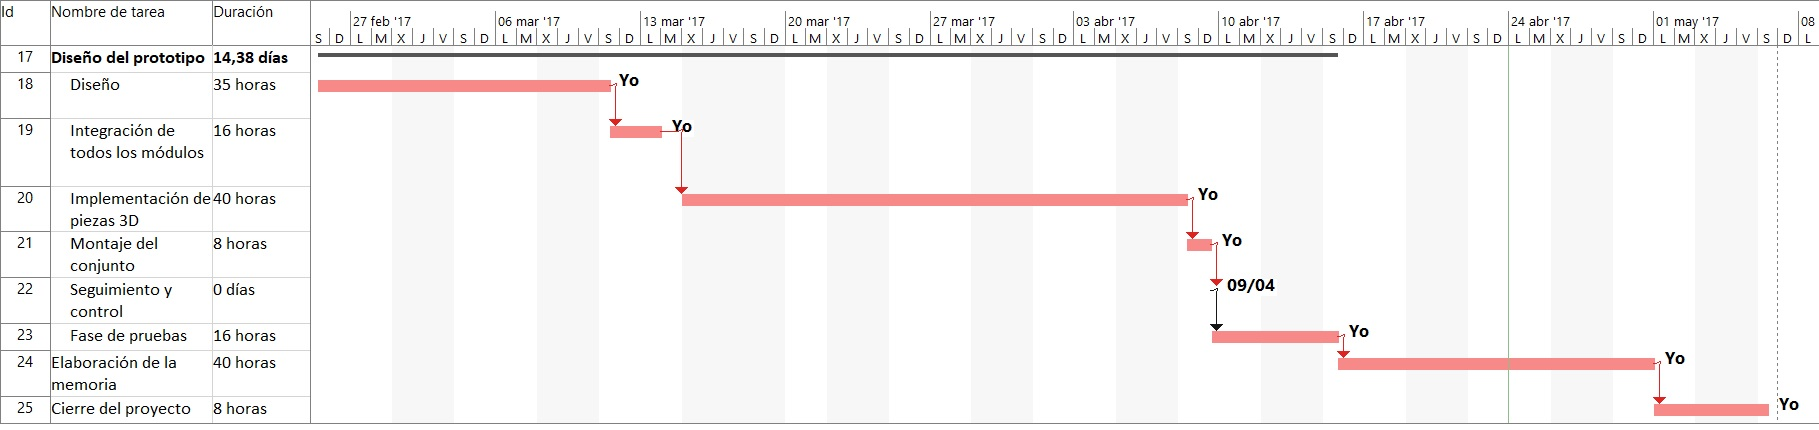
\includegraphics[angle=270,width=0.40\textwidth]{img/ganttInicial_3}
	\caption{Diagrama de Gantt Inicial 3}
	\label{fig:ganttInicial3}
\end{figure}



\section{Planificación financiera inicial} 
A continuación detallaremos una planificación financiera a priori:
\begin{itemize}
    \item Modelo a escala de un buggy: 43,85 \euro
    \item Raspberry Pi 3 modelo B: 38,70 \euro
    \item Variador (control motor): 9,45 \euro
    \item Clavijas conexión motor: 0,35 \euro
    \item Clavija conexión bateria: 1,20 \euro
    \item Webcam: 15 \euro
    \item Cables interconexión: 2 \euro
    \item Horas de trabajo: 389 h * 8 \euro/h = 3112 \euro

\fbox{ Presupuesto total: 3222,55 \euro}
\end{itemize}

\section{Planificación temporal final (real)} 

\section{Planificación financiera final} 

A continuación detallaremos una planificación financiera a posteriori:
\begin{itemize}
	\item Modelo a escala de un buggy: 43,85 \euro
	\item Raspberry Pi 3 modelo B: 38,70 \euro
	\item Webcam: 15 \euro
	\item Variador (control motor): 9,66 \euro
	\item Arduino Nano: 4,40 \euro
	\item Servo: 2,60 \euro
	\item Placa para integrado: 0,37 \euro
	\item Macho-hembra integrado: 0,50 \euro
	\item Macho-macho integrado: 0,50 \euro
	\item Cables integrado: 1,00 \euro
	\item Clavijas conexión motor: 0,35 \euro
	\item Clavija conexión bateria: 1,20 \euro
	\item Cables interconexión: 2 \euro
	\item Placa impresa 3D: 13 \euro
	\item Leds: 2,40 \euro
	\item Resistencias: 0,30 \euro
	\item Horas de trabajo: \euro

\fbox{Presupuesto total: \euro}
\end{itemize}

\section{Estudio de mercado}
\subsection{Clientes potenciales}

	En nuestro proyecto podemos barajar varios clientes potenciales.
	
	\begin{itemize}
		\item Para clientes amantes del modelismo.
		
			Como producto de modelismo podría tener una buena salida ya que es una nueva forma de entender el modelismo. Además suelen ser personas amantes de los nuevos productos, y podría llegar a convertirse en una nueva categoría de este.
			
			
		\item Para clientes a los que les gusta la programación y geeks.
			
			Suponemos que las personas que aquí contemplamos están en los grupos de ``Ciencias, matemáticas e informática'' e ``Ingeniería, industria y construcciones'' ya que son los más propensos a pertenecer a este tipo de clientes. Con ello, según el INE, en el año 2011 estos grupos eran el 8,7 \% y el 16,2 \% de la población respectivamente. Con ello nos da un 24,9 \% de la población que tienen la posibilidad de ser clientes potenciales. \cite{censoINE}
		
		\item Para automatización de coches.
		
			Tomando el censo de conductores de 2015 el número de conductores con el permiso de conducir de tipo B entre una edad de 18 y 40 años es de 7591503. La población en el año 2015 era aproximadamente de 46,62 Millones de personas. Con lo cual supuestamente tendríamos un 16,28 \% de la población que podrían ser clientes potenciales. \cite{censoDGT}
			
		
		\item Para automatización de vehículos extraterrestres.
		
			Alguna de las agencias espaciales podría necesitar este producto al ser un producto de bajo coste y fácilmente escalable y replicable. Podría utilizarse como ``cerebro'' para controlar vehículos que pudiesen ser enviados fuera de la tierra.
			
		
	\end{itemize}

\subsection{Plan de comercialización}

	En nuestro caso vamos a estudiar dos posibles maneras de comercializar el producto.

	\begin{itemize}
		\item Pack automatización
		
			En este caso se vendería las Raspberry, el arduino, la placa que diseñamos y la cámara, además del software que esto incluye. 
			
		\item Coche hobby
		
			Por contra, aquí comercializaríamos el prototipo al completo.
		
	\end{itemize}
 
\cdpchapter{Conclusiones}
\cdpchapter{Trabajo futuro}
\cdpchapter{Bibliografía}
	
	\bibliographystyle{apacite}
	\bibliography{bibliografia} 
	


\cdpchapter{Anexos}

\begin{itemize}
	\item Alojamiento del proyecto
	
		El proyecto ha ido siendo alojado en un repositorio de github para el control de versiones y para tener un respaldo online. Enlace: \url{https://github.com/gorocca/autonomousbuggypi}
	
	\item Videos de prueba
		\begin{itemize}
			\item Primer video de prueba con la aplicación
				\begin{figure}[H]
					\centering
					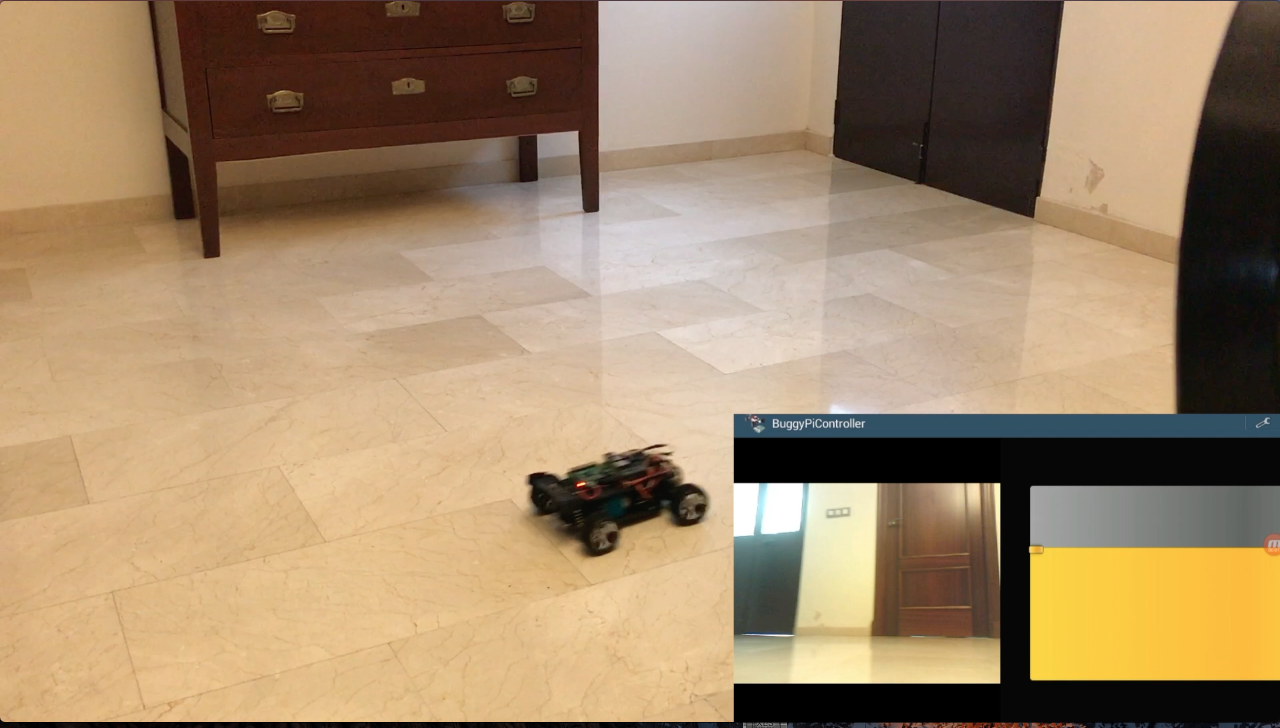
\includegraphics[width=0.7\textwidth]{img/capturaPrimerVideoApp}
					\caption{Captura del video de prueba con la aplicación}
					\label{fig:capturaPrimerVideoApp}
				\end{figure}
		
				 Video: \url{https://youtu.be/g_npEDxkSyo}
				
		\end{itemize}
		
\end{itemize}



\end{document}

